
Um sinal � um conjunto de dados ou informa��es, que podem descrever diversos tipos de fen�menos, como um sinal de telefonia ou de voz (Figura \ref{fig:Voice}), o registro de vendas de uma empresa ou ainda os valores de fechamento de uma bolsa de valores (Figura \ref{fig:CotacaoBovespa}) \cite[p.~75]{Lathi}. Segundo \citeonline[p.~1]{Oppenheim} existe uma linguagem adequada para descrever sinais e um conjunto poderoso de ferramentas para analis�-los, capaz de se aplicar a problemas oriundos de diversos dom�nios. A s�rie de Fourier e a Transformada R�pida de Fourier s�o ambas exemplos destas ferramentas, e ser�o apresentadas nos pr�ximos cap�tulos.

\vspace{5.0mm}

\begin{figure}[H]
	\centering
	\captionsetup{width=0.8\textwidth, font=footnotesize, textfont=bf}	
	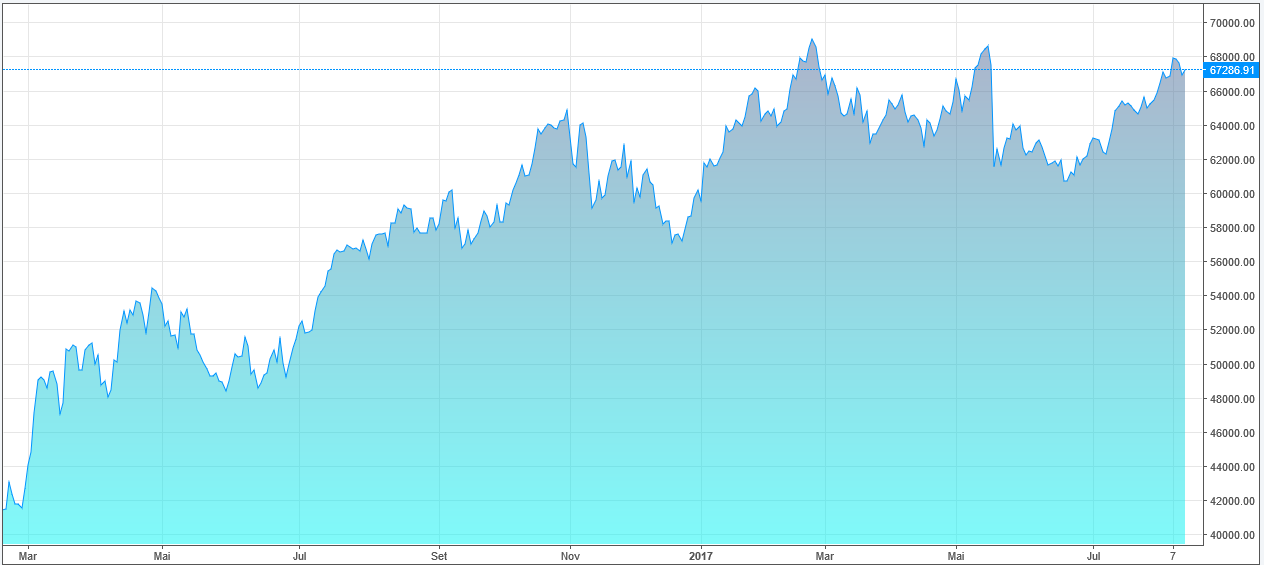
\includegraphics[width=0.8\linewidth]{Images/RevisaoDeLiteratura/CotacaoBovespa.png}
	\caption{�ndice BM \& FBOVESPA, S�o Paulo - Brasil}
	\vspace{-3.5mm}
	\caption*{Fonte: \citeonline{bovespa}}
	\label{fig:CotacaoBovespa}
\end{figure}

\vspace{4mm}

\begin{figure}[H]
	\centering
	\captionsetup{width=0.8\textwidth, font=footnotesize, textfont=bf}	
	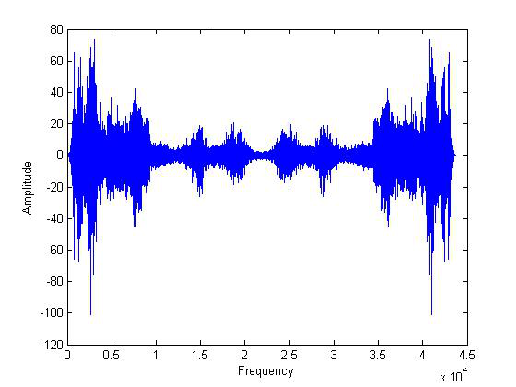
\includegraphics[width=0.8\linewidth]{Images/RevisaoDeLiteratura/Voice.pdf}
	\caption{Sinal Refer�ncia de Voz}
	\vspace{-3.5mm}
	\caption*{Fonte: \citeonline{NirmalRaj}}
	\label{fig:Voice}
\end{figure}

\vspace{4mm}


\section{S�rie de Fourier}
	
A s�rie de Fourier tem como principio os estudos das somas trigonom�tricas de senos e cossenos harmonicamente relacionados,  com o intuito de descrever fen�menos peri�dicos. Tal estudo possui uma longa hist�ria que data pelo menos da �poca dos babil�nicos, e que envolve  o estudo de diferentes fen�menos f�sicos. Mas o marco moderno neste tema ocorre em 1748 com o matem�tico e f�sico su��o Leonhard Paul Euler \cite[p.~104]{Oppenheim}. Euler em seu estudo sobre ondas estacion�rias atrav�s de cordas vibrantes observou que se a configura��o da posi��o vertical $y_0$ de um ponto horizontal $x$ em uma onda estacionaria  no tempo $t_0$ for uma combina��o linear dos modos normais da onda, o mesmo acontece com a configura��o em qualquer valor de tempo $t_s$ subsequente. Com base nesse estudo Euler demonstrou que � poss�vel calcular diretamente os coeficientes da combina��o linear em tempos futuros usando os coeficientes em tempos anteriores. \cite[p.~104]{Oppenheim}.  

\vspace{6mm}
\begin{figure}[H]
	\centering
	\captionsetup{width=0.8\textwidth, font=footnotesize, textfont=bf}	
	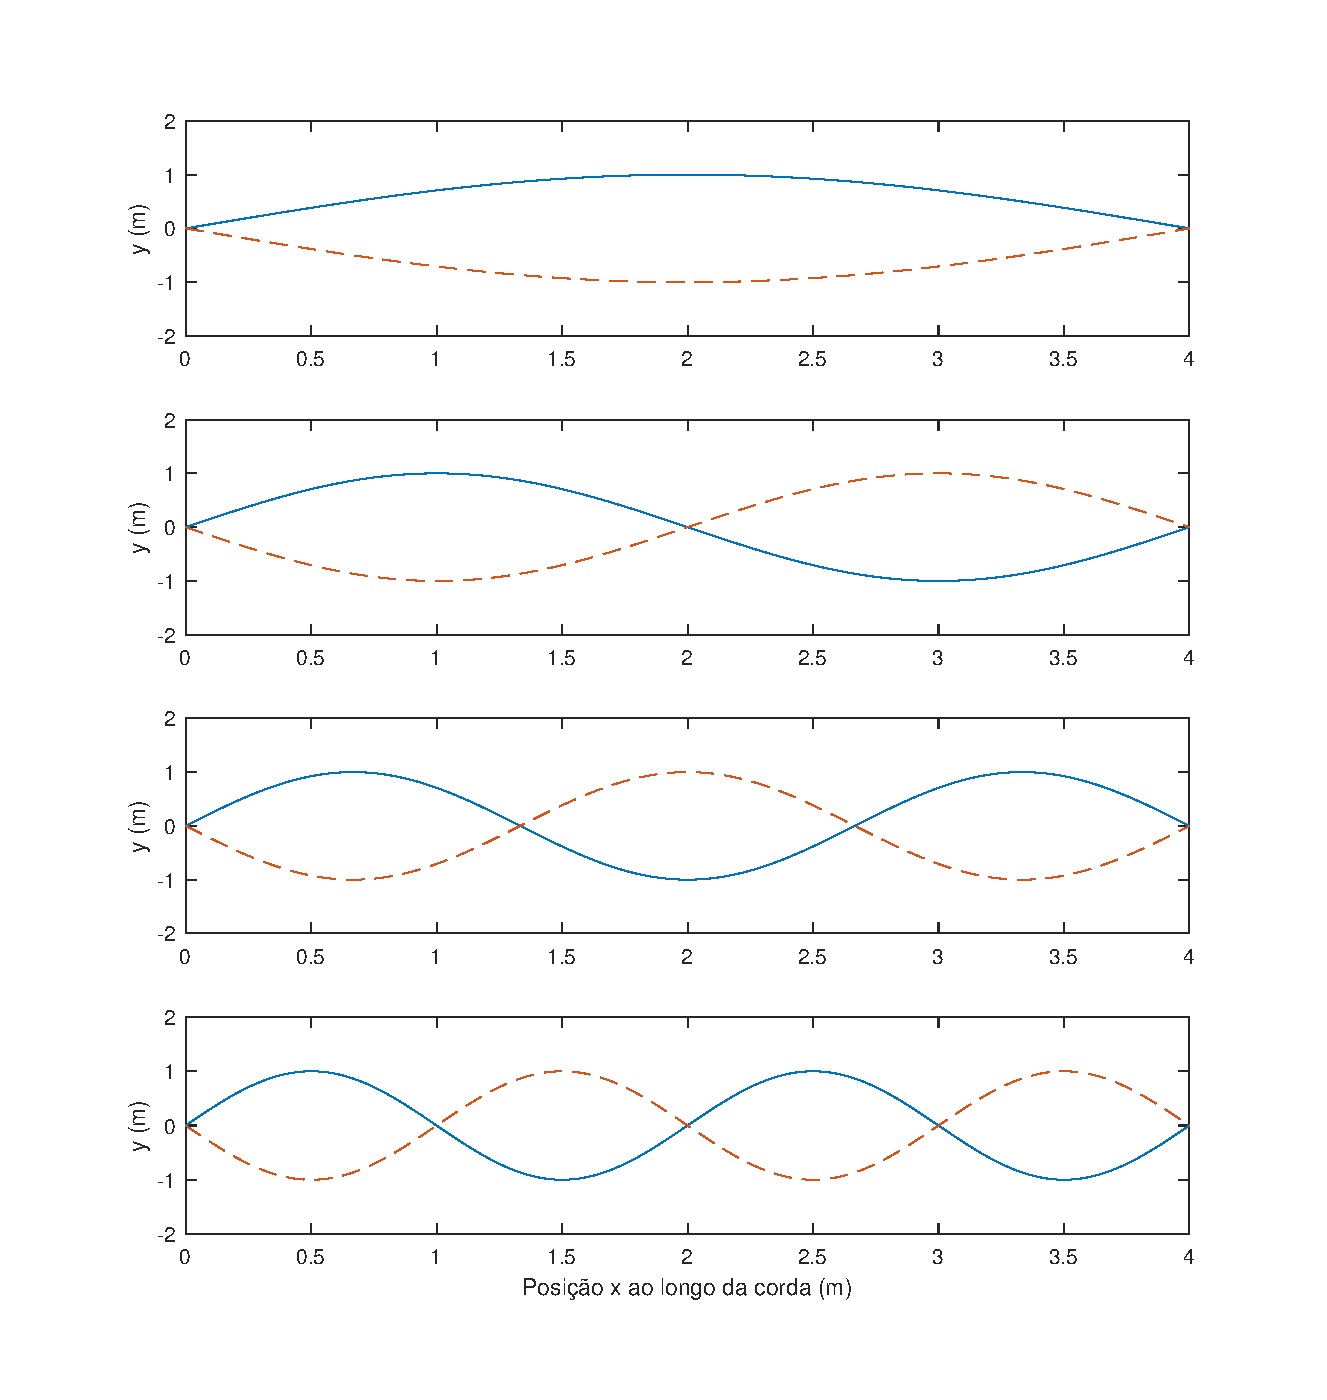
\includegraphics[width=0.8\linewidth]{Images/RevisaoDeLiteratura/OndasEstacionarias.eps}
	\caption{Modos Normais de uma Corda Vibrante}
	\vspace{-3.5mm}
	\caption*{Fonte: Adaptado de \citeonline[p.~105]{Oppenheim}}
	\label{fig:OndasEstacionarias}
\end{figure}
\vspace{6mm}


O estudo de Euler se tornam ainda mais importantes quando aplicado a sinas e a sistemas LIT. Segundo \citeonline[p.~163]{Haykin}, se a entrada de um sistema Linear Invariante no Tempo (LIT) for expressa por uma combina��o linear ponderada de sen�ides ou exponenciais complexas, a sa�da do sistema ser� expressa como uma combina��o linear ponderada da resposta do sistema a cada sen�ide ou exponencial complexa. Expressar sinais em termo de senoides ou exponenciais complexas n�o apenas leva a uma express�o alternativa �til para o comportamento da entrada e sa�da de um sistema LTI, como tamb�m fornece uma caracteriza��o muito criteriosa dos sinais e sistemas. 

Segundo \citeonline[p.~105]{Oppenheim}, meio s�culo depois da divulga��o do trabalho de Euler, o f�sico e matem�tico franc�s Jean-Baptiste Joseph Fourier (1768 - 1830), havia se envolvido no estudo sobre s�ries trigonom�tricas, com a motiva��o f�sica de estudar o fen�meno da propaga��o e difus�o de calor. Fourier conclui que  s�ries senoidais harmonicamente relacionadas eram �teis na representa��o da distribui��o de temperatura em um corpo, e que 'qualquer' sinal peri�dico poderia ser representado po tal s�rie. Fourier ainda apresentou uma representa��o para sinais aperi�dicos, n�o atrav�s de somas ponderadas de senoides harmonicamente relacionadas, mas como integrais ponderadas de senoides que n�o s�o necessariamente harmonicamente relacionadas\cite[p.~163]{Haykin}.

Como afirma \citeonline[p.~106]{Oppenheim}, muitas das ideias b�sica por tr�s das contribui��es de Fourier j� eram conhecidas, e as condi��es precisas sob as quais a representa��o de sinais proposta era v�lida s� foram apresentadas por P.L. Dirichlet em 1829. Por�m foi Fourier que que teve a clara percep��o do potencial pra essa representa��o, e at� certo ponto foi o seu trabalho e suas afirma��es que estimularam grande parte do trabalho subsequente. Logo em sua homenagem o estudo de sinais e sistemas, usando representa��es senoidais, � denominado an�lise de Fourier. E as s�ries pelo qual � realizada a representa��o de sinais na forma de somas de senoides complexas � denominada s�rie de Fourier. 

\subsection{Resposta do Sistemas LTI a Entrada Senoidal} 

Na an�lise de Fourier, os sinais de entrada senoidais s�o comumente usados para caracterizar a resposta de um sistema Linear e Invariante no Tempo, ou LTI (Linear Time-Invariant). A resposta senoidal em estado estacion�rio de um sistema LTI � obtido pela convolu��o entre a entrada senoidal e o sinal de impulso\cite[p.~163]{Haykin}. 

Ao aplicar um sinal impulso ($\delta (t)$) a entrada de um sistema LTI,  � gerado um sinal de sa�da conhecido como resposta ao impulso $\delta (t)$. Atrav�s da resposta ao impulso � poss�vel caracterizar de maneira completa o comportamento de um sistema. A resposta ao impulso tamb�m possibilita conhecer a resposta do sistema LTI a qualquer sinal de entrada, atrav�s da convolu��o deste sinal ao impulso \cite[p.~108]{Haykin}.    

Assim realizando a convolu��o do impulso ao sinal senoidal, segundo \citeonline[p.~164]{Haykin}, a sa�da de um sistema LTI dado uma entrada senoidal complexa $x(t)$, na forma exponencial $e^{j \omega t}$, � dada por:

\begin{equation}
	y(t) = H(j \omega) e^{j \omega t}
	\label{eq:SaidaSenoideComplexa}
\end{equation}

Em que $H(j \omega)$ � a resposta em frequ�ncia, definida em termos de resposta ao impulso $\delta (t)$. Assim;

\begin{equation}
	H(j \omega) = \int_{-\infty}^{\infty} \delta (t) e^{-j \omega t} dt
	\label{eq:RespostaSenoideComplexa}
\end{equation}

Logo a entrada senoidal complexa em um sistema LTI gera uma sa�da igual a entrada senoidal multiplicada apenas pela resposta em frequ�ncia do sistema $H(j \omega)$. 

As equa��es (\ref{eq:SaidaSenoideComplexa}) e (\ref{eq:RespostaSenoideComplexa}) apenas consideram como entrada um sinal senoidal. Por�m � de interesse obter uma express�o para a resposta do sistema LTI a quaisquer sinais arbitr�rios. Para tal \citeonline[p.~164]{Haykin} considera a senoide complexa $\psi~=~e^{j \omega t}$ como uma autofun��o do sistema $H$ associando com o autovalor $\lambda~=~H(j \omega)$, de modo a satisfazer:

\begin{equation}
	H\| \psi \| ~=~ \lambda \psi (t)
\end{equation}

Como pode ser visto na Figura (\ref{fig:PropriedadeDeAutofuncao}), a sa�da de um sistema dada a entrada de uma autofun��o, � o produto da entrada por um n�mero complexo. Se $e_k$ for um autovetor de uma matriz $A$, e $\lambda_k$ os autovalores associados a esta matriz,  a autorrela��o do problema tradicional do autovalor matricial � aplic�vel, $A e_k ~=~ \lambda_k e_k$ \cite[p.~164]{Haykin}.

\vspace{6mm}
\begin{figure}[H]
	\centering
	\captionsetup{width=0.8\textwidth, font=footnotesize, textfont=bf}	
	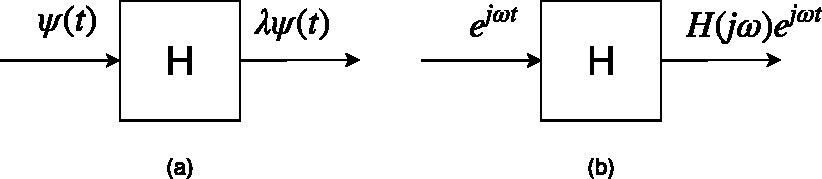
\includegraphics[width=0.8\linewidth]{Images/RevisaoDeLiteratura/PropriedadeDeAutofuncao.pdf}
	\caption{Ilustra��o da Propriedade de Autofun��o de Sistemas Lineares}
	\vspace{-3.5mm}
	\caption*{(a) Autofun��o geral $\psi (t)$ e  autovalor $\lambda$. }
	\vspace{-3.5mm}
	\caption*{(b) Autofun��o senoidal complexa $e^{i \omega t}$ e autovalor $H(j \omega)$.}
	\vspace{-3.5mm}
	\caption*{Fonte: Adaptado de \citeonline[p.~164]{Haykin}}
	\label{fig:PropriedadeDeAutofuncao}
\end{figure} 
\vspace{6mm}

A ideia principal aqui � utilizar a superposi��o ponderada de autofun��es para representar um �nico sinal peri�dico. Para esse efeito \citeonline[p.~164]{Haykin} expressa a entrada de um sistema LTI como uma soma de $N$ senoides complexas ponderadas, na forma: 

\begin{equation}
	x(t) = \sum_{k=1}^{N} a_k e^{j\omega_k t}
\end{equation}

Ou seja na forma de s�rie de Fourier.

Expressar a entrada de um sistema LTI a partir de uma soma ponderada de senoides complexas possui a inten��o de realizar uma aproxima��o coerente do sinal de entrada, utilizando uma composi��o de fun��es b�sicas j� bem conhecidas. Por exemplo considere o sinal de onda quadrada presente na Figura (\ref{fig:AproximacaoPorSomasDeSenoidesA.eps}), o qual deseja-se aproximar utilizando uma soma de senoides complexas. Tomando uma senoide de amplitude 1.286 e uma frequ�ncia de $50Hz$ � poss�vel realizar uma aproxima��o groseira, por�m em fase com este sinal.

\vspace{5mm}
\begin{figure}[H]
	\centering
	\captionsetup{width=0.7\textwidth, font=footnotesize, textfont=bf}	
	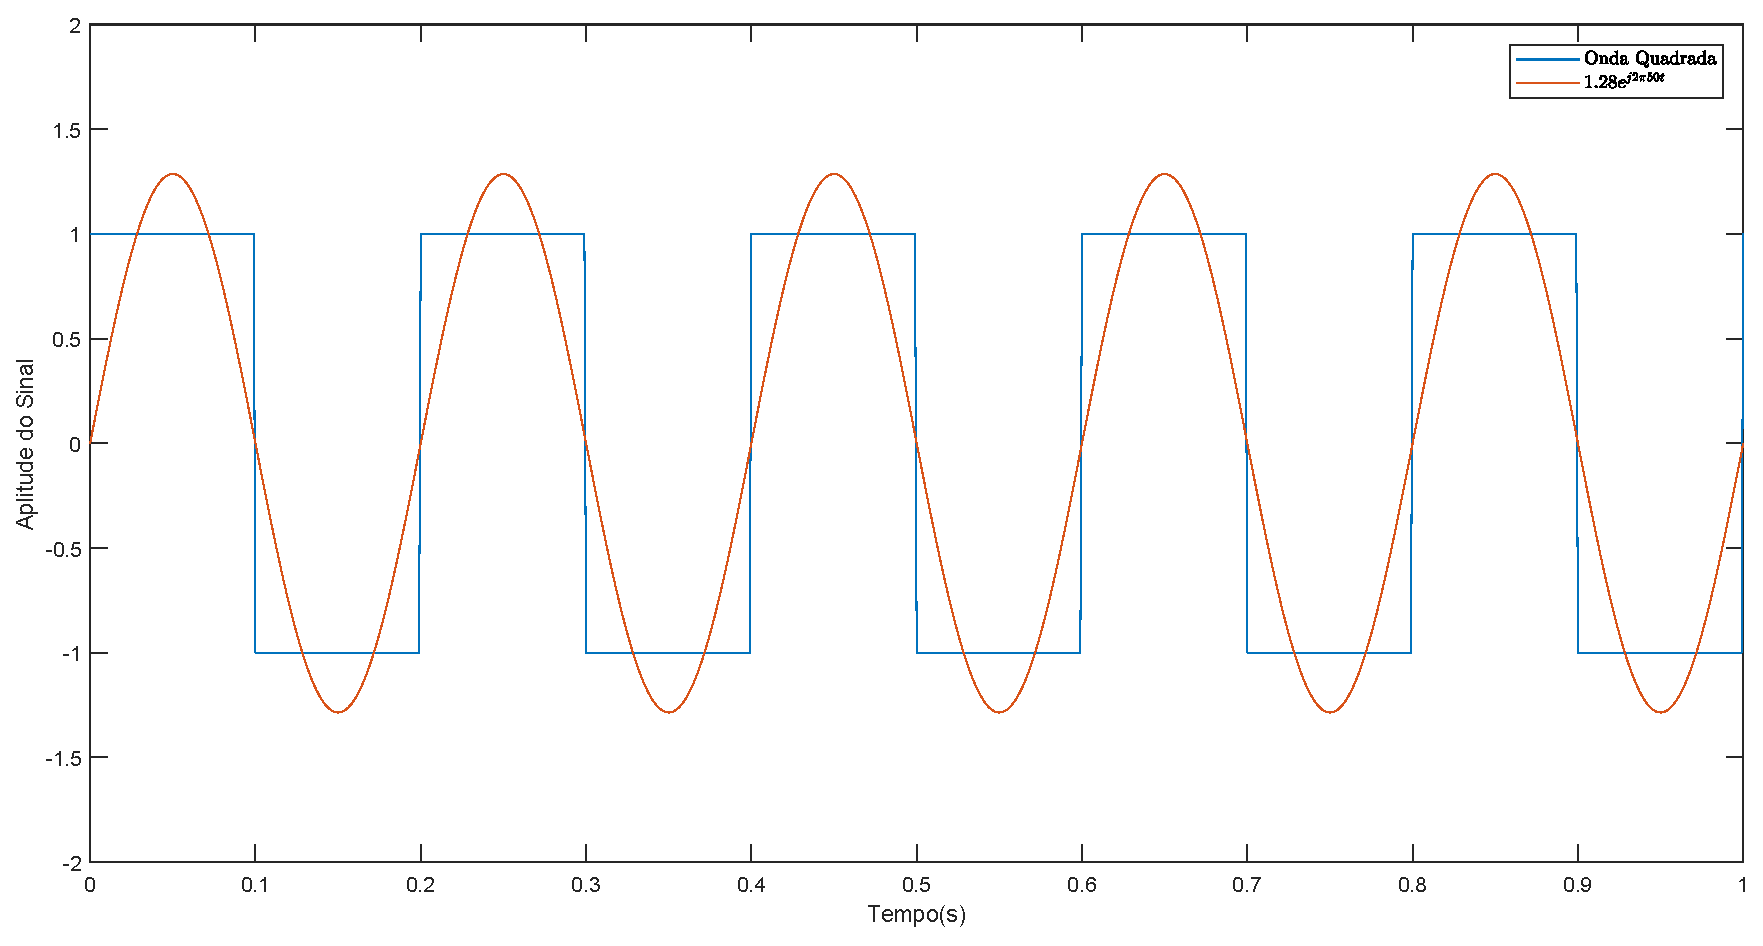
\includegraphics[width=0.7\linewidth]{Images/RevisaoDeLiteratura/AproximacaoPorSomasDeSenoidesA.eps}
	\caption{Aproxima��o do Sinal de Onda Quadrada por um Termo Senoidal}
	\vspace{-3.5mm}
	\caption*{Fonte: Autoria Pr�pria}
	\label{fig:AproximacaoPorSomasDeSenoidesA.eps}
\end{figure}
\vspace{5mm}

Para tornar melhorar a aproxima��o da representa��o em rela��o ao sinal de onda quadrada � poss�vel adicionado mais  termos senoidais ao somat�rio.  Como pode ser visto nas Figura (\ref{fig:AproximacaoPorSomasDeSenoidesB.eps}) e (\ref{fig:AproximacaoPorSomasDeSenoidesC.eps}) as aproxima��es ficam mais suaves adicionando mais 2 ou mais 5 termos respectivamente. Quanto maior o n�mero de termos senoidais complexas ponderados presentes no somat�rio da representa��o maior � a aproxima��o, sendo no limite perfeita.

\vspace{5mm}
\begin{figure}[H]
	\centering
	\captionsetup{width=0.7\textwidth, font=footnotesize, textfont=bf}	
	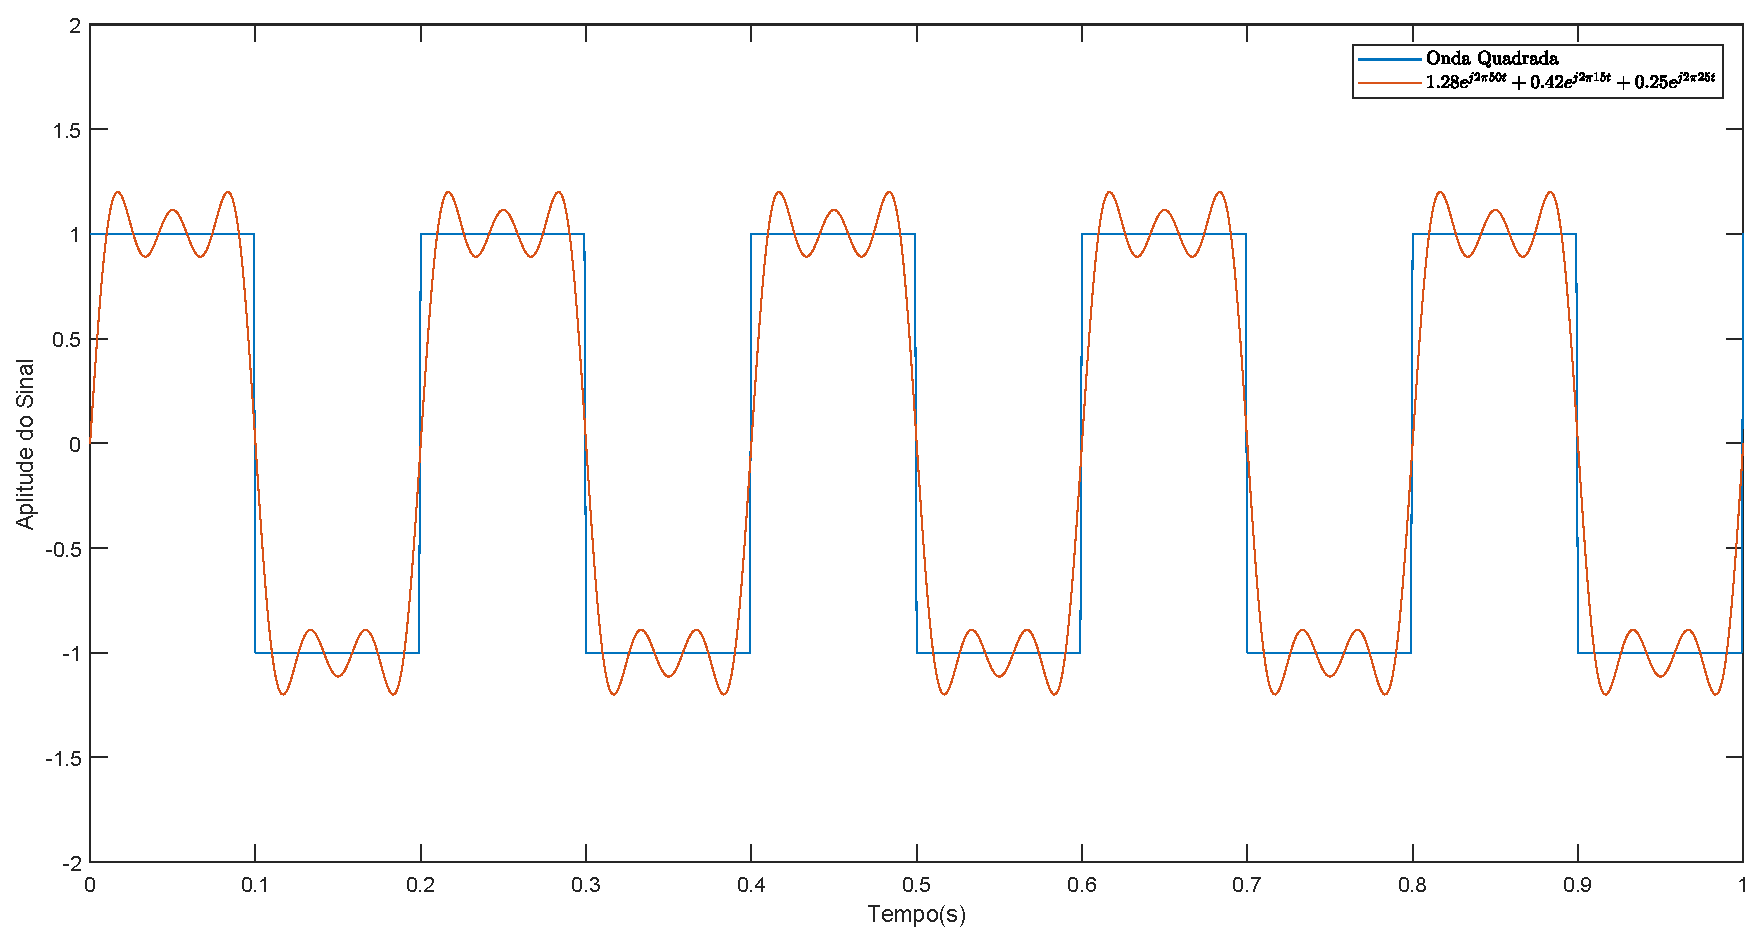
\includegraphics[width=0.7\linewidth]{Images/RevisaoDeLiteratura/AproximacaoPorSomasDeSenoidesB.eps}
	\caption{Aproxima��o do Sinal de Onda Quadrada por Soma de 3 Termos Senoidais}
	\vspace{-3.5mm}
	\caption*{Fonte: Autoria Pr�pria}
	\label{fig:AproximacaoPorSomasDeSenoidesB.eps}
\end{figure}
\vspace{5mm}
\begin{figure}[H]
	\centering
	\captionsetup{width=0.7\textwidth, font=footnotesize, textfont=bf}	
	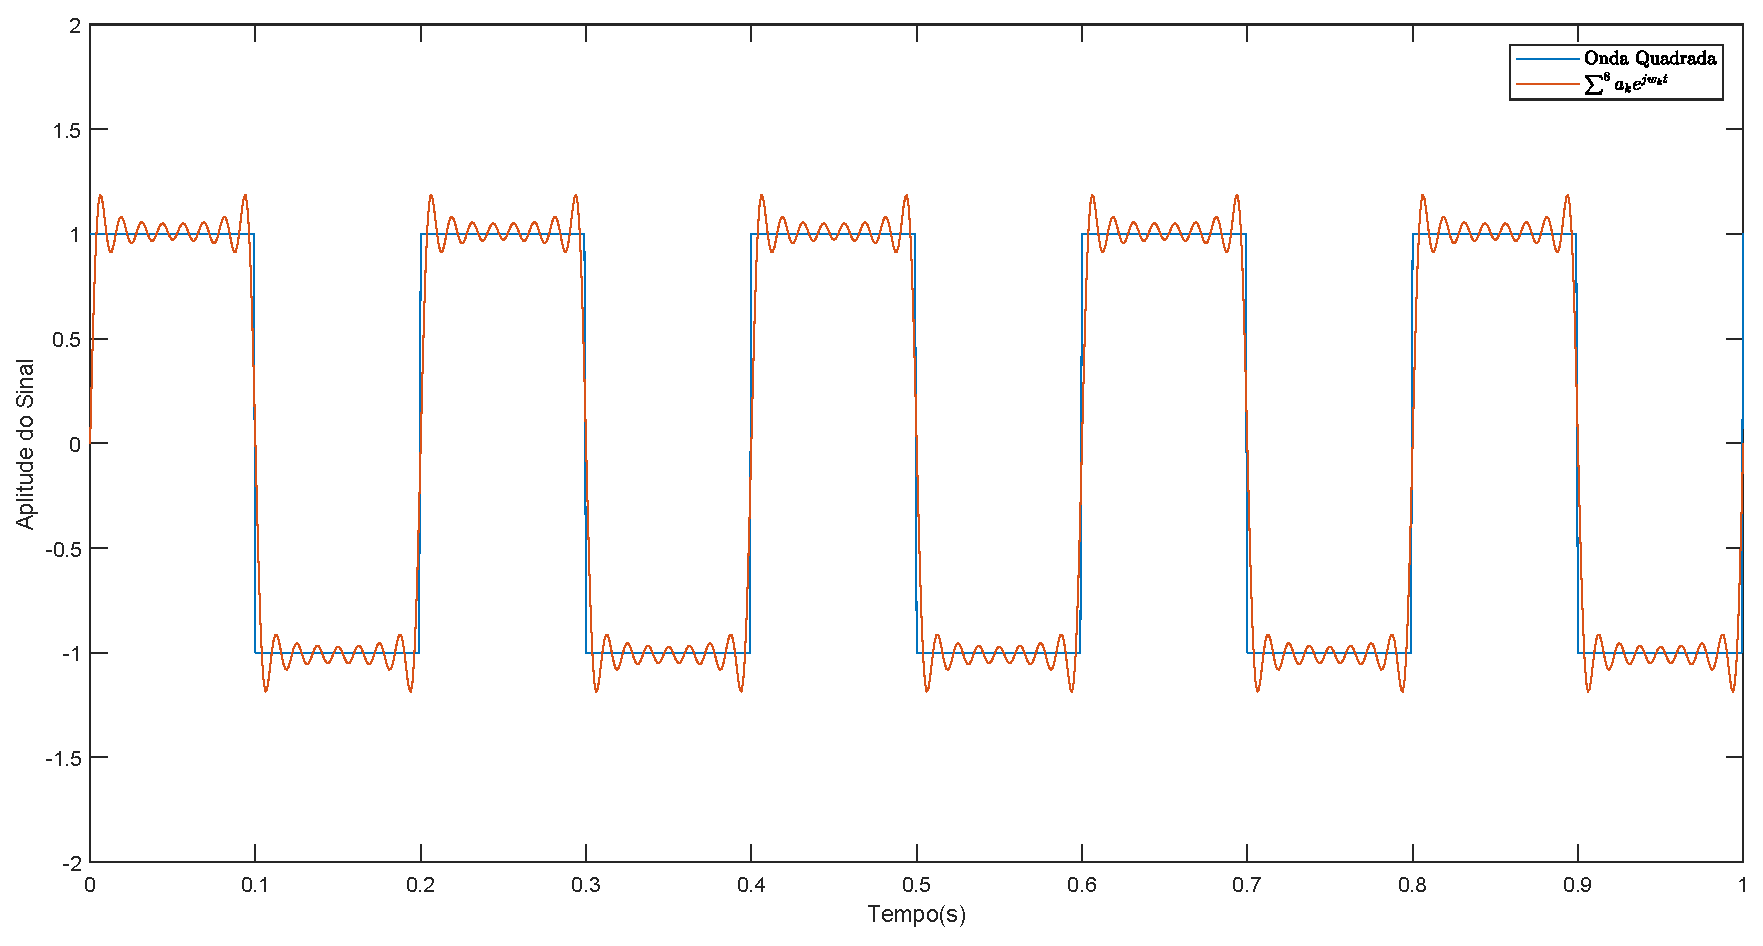
\includegraphics[width=0.7\linewidth]{Images/RevisaoDeLiteratura/AproximacaoPorSomasDeSenoidesC.eps}
	\caption{Aproxima��o do Sinal de Onda Quadrada por Soma de 8 Termos Senoidais}
	\vspace{-3.5mm}
	\caption*{Fonte: Autoria Pr�pria}
	\label{fig:AproximacaoPorSomasDeSenoidesC.eps}
\end{figure} 
\vspace{5mm}

Logo utilizando se $e^{j\omega_k t}$ for uma autofun��o e $H(j\omega_k)$ for o autovalor do sistema, aplicando-se a autorrela��o apresentada anteriormente, o sinal de sa�da do sistema e dado por:

\begin{equation}
	y(t) = \sum_{k=1}^{N} a_k H(j\omega_k)e^{j\omega_k t}
\end{equation}

A sa�da, portanto nada mais � do que a soma ponderada das senoides complexas da entrada, sendo os pesos $a_k$ ponderados pela resposta em frequ�ncia $H(j\omega_k)$. Por meio deste resultados � poss�vel transformar a opera��o de convolu��o em uma opera��o de multiplica��o dos termos $a_k~H(j\omega_k)$. Segundo \citeonline[p.~164]{Oppenheim} o fato da sa�da de um sistema LTI dada uma entrada representada como combina��o linear de senoides complexas, ser tamb�m uma combina��o linear dos mesmos sinais, foi uma descoberta de Euler, que motivou Fourier e os outros matem�ticos ap�s ele no estudo da extens�o de classes de sinais que poderiam ser representados nesta forma de somat�rios de exponenciais complexas ponderadas.

Al�m de tornar mais pr�tico o c�lculo da convolu��o de sinais, a representa��o em somais senoidais complexas ponderadas fornece uma interpreta��o alternativas para sinais e sistemas  \citeonline[p.~166]{Haykin}. Atrav�s da an�lise dos pesos  $a_k$ ponderados � poss�vel descrever um sinal em fun��o da frequ�ncia, ao inv�s do tempo. 

A representa��o de sinais por s�ries de Fourier pode ser aplicada para diferentes tipos de sinais, com diferentes caracter�sticas. H� quatro classes de representa��es de  Fourier, dividias de acordo com a sua periodicidade e sua continuidade, como poder ser visto na Tabela \ref{tab:PropriedadeTempoERepresentacaoFourier}. 

Para sinais peri�dicos a representa��o � feita como s�ries de Fourier, sendo que para sinais de tempo continuo � aplicado a S�rie de Fourier (FS - \textit{Fourier Series}), e para sinais de tempo discreto � usada as s�ries de Fourier de tempo discreto (DFS - \textit{Discrete Fourier Serie}). Quando os sinais n�o s�o peri�dicos a representa��o � denominada como transformada, para o caso do sinal ser cont�nuo a representa��o � feita pela transformada de Fourier (FT - \textit{Fourier Transform}), e no caso discreto � a transformada de Fourier de tempo discreto (DFT - \textit{Discrete Fourier Trasform}).

\vspace{6mm}
\begin{table}[h]
\centering
\captionsetup{width=0.9\linewidth}
\begin{tabular}{|c|c|c|}
	\hline
	Propriedade do Tempo                                                      & \cellcolor[HTML]{000000}{\color[HTML]{FFFFFF} Peri�dico} & \cellcolor[HTML]{000000}{\color[HTML]{FFFFFF} N�o Periodico} \\ \hline
	\cellcolor[HTML]{000000}{\color[HTML]{FFFFFF} }                           & S�rie de Fourier (FS)                                    & Transformada de                                              \\
	\multirow{-2}{*}{\cellcolor[HTML]{000000}{\color[HTML]{FFFFFF} Continuo}} & \multicolumn{1}{l|}{}                                    & Fourier (FT)                                                 \\ \hline
	\cellcolor[HTML]{000000}{\color[HTML]{FFFFFF} }                           & S�rie de Fourier de                                      & Transformada de Fourier de                                   \\
	\multirow{-2}{*}{\cellcolor[HTML]{000000}{\color[HTML]{FFFFFF} Discreto}} & \multicolumn{1}{l|}{Tempo Discreto (DFS)}                & \multicolumn{1}{l|}{Tempo DIscreto (DFT)}                    \\ \hline
\end{tabular}
\caption{Rela��o entre propriedade do tempo de um sinal e a representa��o de Fourier adequada}
\vspace{-3.5mm}
\caption*{Fonte: \citeonline[p.~166]{Oppenheim}}
\label{tab:PropriedadeTempoERepresentacaoFourier}
\end{table}
\vspace{6mm}

A representa��o de Fourier utilizada no desenvolvimento deste trabalho � a DFT, e portanto a mais importante a ser apresentada. As pr�ximas se��es deste trabalho passaram pela apresenta��o da FS depois pela DFS para em fim chegar na DFT. 

\subsection{S�rie de Fourier}

Segundo \citeonline[p.~530]{Lathi}  "Um sinal peri�dico $x(t)$ com per�odo $T_0$ pode ser descrito como a soma de senoides de frequ�ncia $f_0$ e todas as suas harm�nicas", conforme apresentado na Equa��o (\ref{eq:SerieFourierFundamental}). Esta � a chamada s�rie de Fourier para sinais peri�dicos, ou apenas s�rie de Fourier. Na express�o da Equa��o (\ref{eq:SerieFourierFundamental}) a s�rie de Fourier est� na forma trigonom�trica. Onde $\omega_0$ � a frequ�ncia fundamental de $x(t)$, e $a_0$, $a_n$ e $b_n$ s�o os coeficientes de amplitude das harm�nicas que comp�es $x(t)$, sendo $a_0$ a harm�nica zero (n�vel CC).


\begin{equation}
	x(t) ~=~ a_0 + \sum _{n=1} ^{\infty} a_n cos (n \omega_0 t) + b_n sen(n \omega_0 t)
	\label{eq:SerieFourierFundamental}
\end{equation}

Os coeficientes $a_0$, $a_n$ e $b_n$ da Equa��o (\ref{eq:SerieFourierFundamental} ) s�o determinados pelas seguintes equa��es: 

\begin{equation}
	a_0~=~\frac{1}{T_0} \int_{T_0} x(t) dt
	\label{eq:SerieFourierFundamentala0}
\end{equation}

\begin{equation}
	a_n~=~\frac{2}{T_0} \int_{T_0} x(t) cos(n \omega_0 t) dt
	\label{eq:SerieFourierFundamentalan}
\end{equation}

\begin{equation}
	b_n~=~\frac{2}{T_0} \int_{T_0} x(t) sen(n \omega_0 t) dt
	\label{eq:SerieFourierFundamentalbn}
\end{equation}

em que $T_0$ representa o per�odo relativo a frequ�ncia fundamental $f_0$.

� s�rie de Fourier, al�m da forma trigonom�trica, tamb�m pode ser apresentada na forma  exponencial, em termos de $e^{j \omega_0 t}$, como apresentado na se��o anterior. A forma exponencial, segundo \citeonline[p.~533]{Lathi}, � dada atrav�s da Equa��o (\ref{eq:SerieFourierExponencial}), em que o coeficiente $C_n$ e an�logo aos coeficientes $a_n$ e $b_n$ da serie trigonom�trica, sendo obtido por (\ref{eq:SerieFourierExponencialCn}) .

\begin{equation}
	x(t)~=~\sum^{\infty} _{- \infty} C_n e^{j n \omega_0 t}
	\label{eq:SerieFourierExponencial}
\end{equation}

\begin{equation}
	C_n~=~ \frac{1}{T_0} \int_{T_0} x(t) e^{j n \omega_0 t} dt
	\label{eq:SerieFourierExponencialCn}
\end{equation}

Tanto a forma trigonom�trica quanto a exponencial da s�rie de Fourier consideram $x(t)$como sendo uma fun��o qualquer, real ou complexa. Por�m na maioria das aplica��es $x(t)$ � real, como � o caso dos sinais neste trabalho. Segundo segundo \citeonline[p.~533]{Lathi}, se o sinal de entrada do sistema LTI $x(t)$ � real, isso significa que $a_n$ e $b_n$ tamb�m s�o reais para todos os valores de $n$, sendo portanto a s�rie  de Fourier representada na forma compacta:

\begin{equation}
	x(t) = D_0 + \sum_{n=1}^{\infty} D_n cos(n \omega_0 t + \theta_n)
	\label{eq:FourierCompact}
\end{equation}

Sendo:

\begin{equation}
	D_0 = a_0
\end{equation}

\begin{equation}
	D_n = \sqrt{a_n^2 + b_n^2}
\end{equation}

\begin{equation}
	\theta_n = tan^{-1} \frac{-b_n}{a_n}
\end{equation}

Utilizar $cos $

\subsection{Espectro de Fourier}

Por meio da s�rie de Fourier na forma compacta, apresentada na Equa��o \ref{eq:FourierCompact}, conclui-se que um sinal real peri�dico $x(t)$ pode ser descrito como uma soma de senoides de frequ�ncias $n \omega_0$ e amplitudes $D_n$ e fases $\theta_n$. Segundo \citeonline[p.~533]{Lathi}, o espectro exponencial de Fourier � tra�ado a partir de $D_n$ e $\theta_n$ em fun��o das frequ�ncias $n \omega_0$. Logo s�o ta�ados dois gr�ficos para o espectro exponencial de Fourier, um que relaciona $C_n$ com $n \omega_0$, chamado espectro de magnitude. E outro que relaciona $\theta_n$ com $n \omega_0$, chamado de espectro de fase.

Tomando como exemplo um sinal $x(t)~=~sin(2 \pi 15t) + sin(2\pi40t)$, expresso em um per�odo igual a 1 segundo, como mostrado na Figura \ref{fig:EspectroDeFourier}. Para este sinal e expresso o espectro de Fourier na mesma Figura (\ref{fig:EspectroDeFourier}), com o espectro de magnitude e fase. 

\vspace{5mm}
\begin{figure}[H]
	\centering
	\captionsetup{width=0.9\textwidth, font=footnotesize, textfont=bf}	
	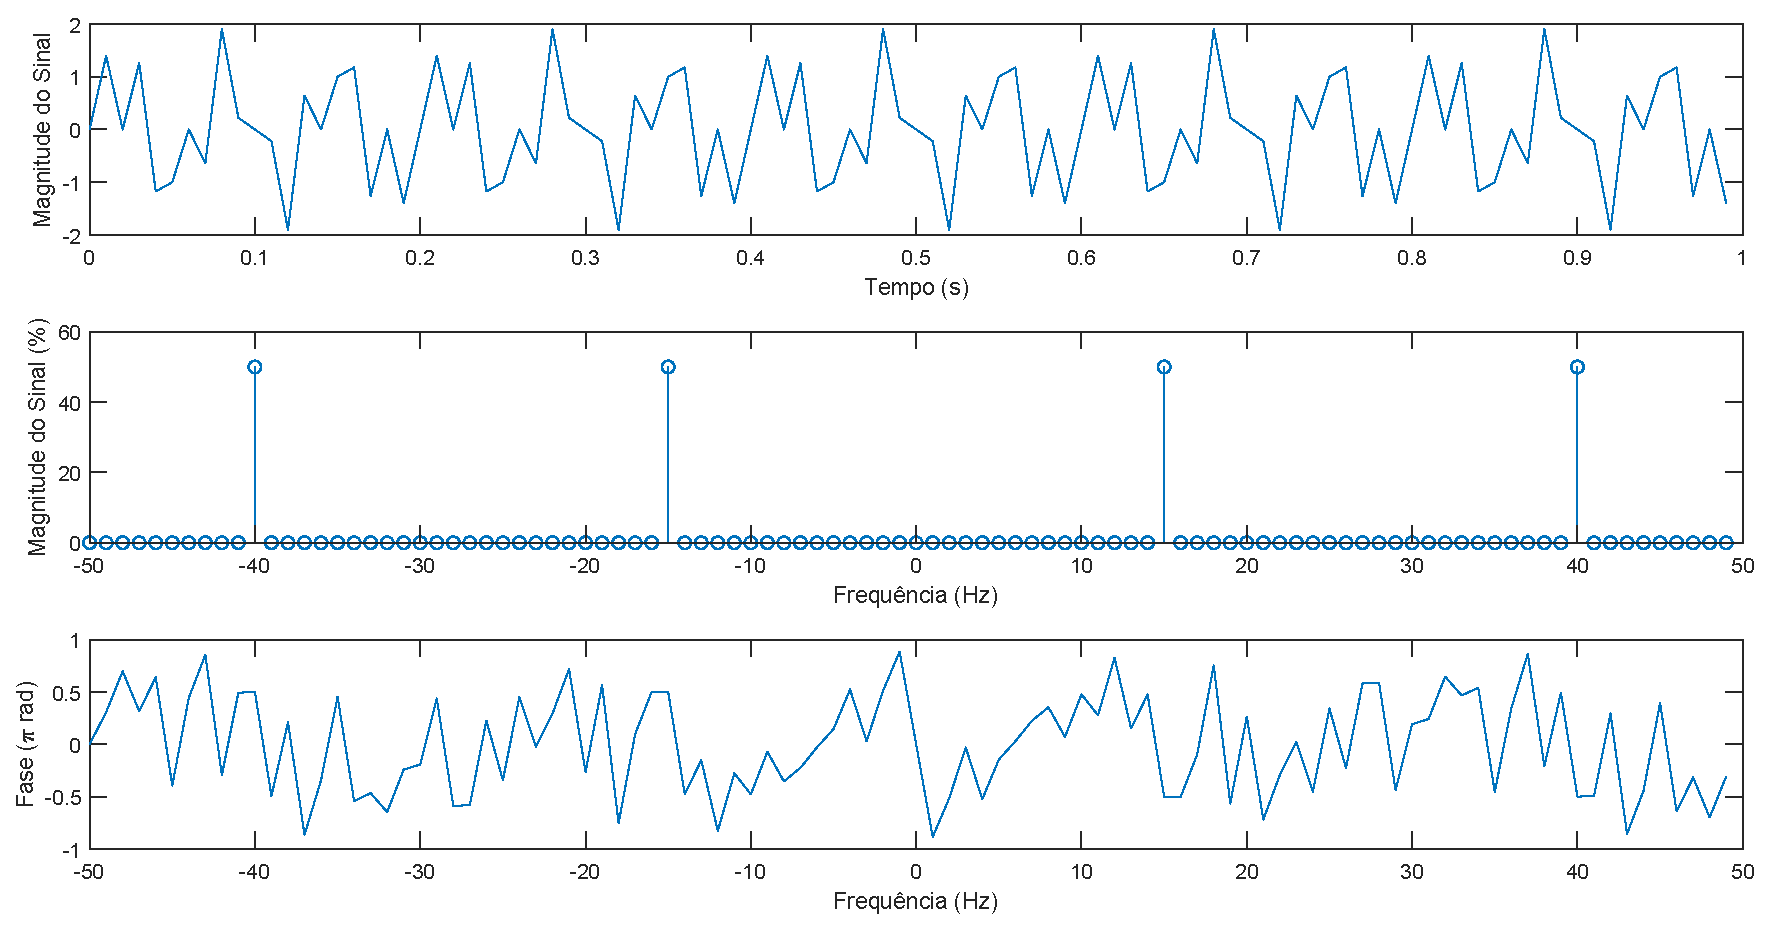
\includegraphics[width=0.9\linewidth]{Images/RevisaoDeLiteratura/EspectroDeFourier.eps}
	\caption{Aproxima��o do Sinal de Onda Quadrada por Soma de 8 Termos Senoidais}
	\vspace{-3.5mm}
	\caption*{Fonte: Autoria Pr�pria}
	\label{fig:EspectroDeFourier}
\end{figure} 
\vspace{5mm}

Nota-se que o espectro da Figura  (\ref{fig:EspectroDeFourier}) aparecem frequ�ncias negativas, as quais dividem a magnitude com suas frequ�ncias sim�tricas. Isso ocorre devido a simetria do angulo $n \omega_0 t$ possui no calculo dos coeficientes da s�rie de Fourier. Para resolver este problema basta considerar apenas a parte positiva do espectro e multiplicar por 2 a magnitude das frequ�ncias no espectro de magnitude. 

Para \citeonline[p.~533]{Lathi} os dois gr�ficos de magnitude e fase juntos formam o espectro de frequ�ncia, o qual revela os conte�dos de frequ�ncia do sinal $x(t)$, com suas amplitudes e fase. Conhecendo-se este espectro n�o s� � poss�vel analisar o sinal $x(t)$ dentro do dom�nio da frequ�ncia, como tamb�m reconstru�-lo de forma f�cil .

	
\section{S�rie de Fourier em Tempo Discreto}
	Ate aqui foi apresentada a forma continua da s�rie de Fourier, por�m para ser �til em uma aplica��o computacional � necess�rio encontrar sua forma discreta, ou DFT \textit{(Discrete Fourier Transform)}. Segundo HAYKIN e Veen (2001, p. 314) a DFT �
a �nica representa��o de Fourier que pode ser calculada por um computador, sendo amplamente usada para manipular sinais.

O primeiro passo para se obter uma DFT e considerar o teorema da Amostragem. Tal teorema afirma que um sinal real $x(t)$, cujo o espectro e limitado em $\phi~Hz$, pode ser reconstru�do a partir de suas amostras tomadas uniformemente a uma taxa $f_s \textgreater 2 \phi$ \cite[p.~679]{Lathi}. Em seguida, a amostragem de $x(t)$, feita a
uma frequ�ncia $f_s$, pode ser obtida pela multiplica��o de $x(t)$ por um trem de impulsos $\delta (t)$. Sendo tais impulsos unit�rios e peri�dicos, repetidos a cada  $T~=~1/f_s$ segundos, por um numero total de amostras $N_0$, a amostragem pode ser definida por:

\begin{equation}
	\overline{x}(t)~=~x(t) \delta_{T}(t)~=~\sum^{N_0 -1} _{n=0} x(nT) \delta(t-nT)
	\label{eq:FourierAmostragem}
\end{equation}

Por conveni�ncia, deseja-se obter um espectro do sinal amostrado $x(t)$ em fun��o de $\omega$ ou expresso em termos de frequ�ncia. Para tal, segundo \citeonline[p.~681]{Lathi}, o trem de impulsos $\delta(t)$ e um sinal peri�dico que pode ser descrito pela s�rie trigonom�trica de Fourier da seguinte forma:

\begin{equation}
	\delta_T (t)~=~\frac{1}{T} [1+ 2cos(\omega_s t) + 2cos(2\omega_s t) + 2cos(3\omega_s t) + \dotsc]
	\label{eq:TremDeImpulsos}
\end{equation}

Logo, multiplicando $x(t)$ por $\delta_{T} (t)$, obtem-se:

\begin{equation}
	\overline{x}(t)~=~x(t) \delta_{T}(t)~=~\frac{1}{T} [x(t) + 2x(t)cos(\omega_s t) + 2x(t)cos(2 \omega_s t) + 2x(t)cos(3 \omega_s t) + \dotsc]
	\label{eq:FourierAmostragemTremDeImpulsos}
\end{equation} ?

Segundo \citeonline[p.~125]{Oppenheim}, a transformada de Fourier do primeiro termo $x(t)$, em (\ref{eq:FourierAmostragemTremDeImpulsos}), � $X(\omega)$. J� a transformada de Fourier do segundo termo 2x(t)cos(!st) � $X(\omega ? \omega_s)~+~X(\omega + \omega_s)$, e do terceiro termo $2x(t)cos(2 \omega_s t)$ �
$X(\omega ? 2 \omega_s) + X(\omega + 2 \omega_s)$. E assim, semelhantemente a transformada de Fourier dos demais termos da serie que descreve (\ref{eq:FourierAmostragemTremDeImpulsos}), representam o espectro $X(\omega)$ deslocado em $n\omega_s$ e $?n\omega_s$. Assim,

\begin{equation}
	\overline{X}( \omega )~=~ \frac{1}{T} \sum_{\infty}^{-\infty} X(\omega - n \omega_s)
	\label{eq:FourierAmostragemDeslocada}
\end{equation}

Desde que a frequ�ncia de amostragem $f_s$ garanta o crit�rio do teorema da Amostragem, o sinal $\overline{X}$ ser� constitu�do de repeti��es n�o sobrepostas de $x(\omega_0)$, a um intervalo de tempo $T = 1/f_s$. Logo tanto $\overline{X}(\omega)$, quanto $\overline{x}(t)$ s�o peri�dicas e equivalentes, por�m com representa��es distintas do especto amostrado. Sendo assim, atrav�s da propriedade de deslocamento no tempo da transformada de Fourier (\ref{eq:Impulso}) e da e (\ref{eq:FourierAmostragem}), obt�m-se (\ref{eq:FourierAmostragemExponencial}) \citeonline[p.~125]{Oppenheim}:

\begin{equation}
	\delta(t - nT) \longleftrightarrow e^{-jn \omega T }
	\label{eq:Impulso}
\end{equation}

\begin{equation}
	\overline{x}(t)~=~\sum_{n=0}^{N_0 - 1} x(nT)e^{-j n \omega T}
	\label{eq:FourierAmostragemExponencial}
\end{equation}

Segundo \citeonline[p.~705]{Lathi}, a transformada de $\overline{x}(t)$ pode ser aproximada, considerando um certo \textit{aliasing} negligenci�vel, para $X(\omega)/T$. Portanto:

\begin{equation}	
	X(\omega)~=~T \sum_{n=0}^{N_0 - 1} x(nT) e^{j n \omega T} ~~ |\omega| \leq \frac{\omega_s}{2}
	\label{eq:DefinicaoDFT}	
\end{equation}

Analisando a propriedade peri�dica de $x(t)$ e $X(\omega)$, e considerando $x(nT)$ e $X(r\omega_0)$ a n-�sima e r-�sina amostra de $x(t)$ e $X(\omega)$, respectivamente, s�o definidas as seguintes vari�veis:

\begin{equation}
	x_n~=~Tx(nT)
	\label{eq:DefinicaoDFTA}
\end{equation}

\begin{equation}
	x_n~=~\frac{T_0}{N_0}x(nT)
	\label{eq:DefinicaoDFTB}
\end{equation}

\begin{equation}
	X_r ~=~ X ( \omega )
	\label{eq:DefinicaoDFTC}
\end{equation}

\begin{equation}
	\omega~=~r \omega_0
	\label{eq:DefinicaoDFTD}
\end{equation}

\begin{equation}
	X_r~=~X(r \omega_0)
	\label{eq:DefinicaoDFTE}
\end{equation}

\begin{equation}
	\omega_0~=~2 \pi f_0 ~=~\frac{2 \pi}{T_0}
	\label{eq:DefinicaoDFTF}
\end{equation}

Assim, substituindo (\ref{eq:DefinicaoDFTE}) e (\ref{eq:DefinicaoDFTB}) em (\ref{eq:DefinicaoDFT}), e fazendo $\omega_0 T = \Omega_0 = 2 pi /N_0$, se
obt�m a seguinte express�o para a transformada discreta de Fourier \cite[p.~125]{Oppenheim}:

\begin{equation}
	X_r~=~\sum_{n=0}^{N_0 - 1} x_n e^{j \omega_0 n r}
	\label{eq:DefinicaoDFTG}
\end{equation}

Onde:

\begin{equation}
	\Omega_0~=~\frac{2 \pi}{N_0}
	\label{eq:DefinicaoOmega}
\end{equation}

Para compactar a express�o de (\ref{eq:DefinicaoDFTG}) se faz a substitui��o da express�o exponencial pela vari�vel  $W$, de modo que $W_{N_0} = e^{?2 \pi /N_0} = e^{-j \Omega_0}$. Logo a express�o para DFT � dada por (\ref{eq:DFT}) \cite[p.~344]{meyer}:

\begin{equation}
	X_r~=~\sum_{n=0}^{N_0 - 1} x_n e^{j \omega_0 n r}
	\label{eq:DFT}
\end{equation}

Onde:

\begin{equation}
	0 \leq k  \leq N_0 - 1
	\label{eq:N0}
\end{equation}


	
\section{Transformada R�pida de Fourier}
	
Para se calcular uma DFT de $N_0$ valores usando apenas (\ref{eq:DFT}), � necess�rio realizar um total de $N^2_0$ multiplica��es e  $N_0(N_0 - 1)$ somas, utilizando n�meros complexos. Deste modo, quando $N_0$ assume um valor elevado, muitos recursos computacionais s�o necess�rios, at� chegar ao ponto de que esse algoritmo se torna impratic�vel.

A redu��o do numero de opera��es matem�ticas necess�rias para calcular a DFT � poss�vel a partir do algoritmo criado por J.W. Cooley e John Tukey, conhecido como Transformada R�pida de Fourier ou FFT \textit{(Fast Fourier Transform)} \citeonline[p.~719]{Lathi}. Para reduzir o numero de c�lculos, a FFT se utiliza da propriedade linear da transformada de Fourier. Segundo \citeonline[p.~119]{Oppenheim}, a transformada de Fourier de um sinal pode ser dada pela combina��o linear da transformada de Fourier de segmentos menores do mesmo sinal. Logo, � poss�vel aplicar a DFT o paradigma da Divis�o e Conquista, o qual � um recurso muito utilizado em algoritmos de ordena��o. 

Segundo \citeonline[p.~21]{Cormen}, um algoritmo de Divis�o e Conquista realiza o desmembramento de um problema em v�rios subproblemas que s�o id�nticos ao original, por�m menores em sua faixa de a��o, o que os torna mais simples de resolver. Em seguida, resolvem-se os subproblemas recursivamente e combinam-se essas solu��es de modo a obter a solu��o para o problema original.

De modo muito semelhante, o algoritmo da FFT prev� uma divis�o recursiva  da DFT em dois blocos: bloco par e o bloco �mpar, como mostrado abaixo\cite[p.~35]{Chu}: 

\begin{equation}
	X_r~=~\underbrace{\sum^{\frac{N_0}{2} - 1}_{n=0} x_{2n} W^{2nr}_{N_0}}_{Parcela~Par} ~ + ~\underbrace{\sum^{\frac{N_0}{2} - 1}_{n=0} x_{2n+1} W^{(2n+1)r}_{N_0}}_{Parcela~\acute{I}mpar}.
	\label{eq:DenicaoFFT}  
\end{equation}

Nesta mesma equa��o os limites dos somat�rios de ambas as parcelas �mpar e par foram redefinidas para englobar apenas metade dos $N_0$ pontos, bem como os expoentes de $W$ foram ajustados.

Utilizando algumas das propriedades geom�tricas de $W$, j� que este representa um numero complexo, pode-se realizar simplifica��es importantes em \ref{eq:DenicaoFFTA}. Primeiro, nota-se que $W_{N_0 / 2}~=~W_{N_0} ^{2}$, logo:

\begin{equation}
	X_r~=~\underbrace{\sum^{\frac{N_0}{2} - 1}_{n=0} x_{2n} W^{2nr}_{N_0}}_{G_r} ~ + ~\underbrace{\sum^{\frac{N_0}{2} - 1}_{n=0} x_{2n+1} W^{(2n+1)r}_{N_0}}_{H_r}.
	\label{eq:DenicaoFFTA}  
\end{equation}

Como $G_r$ e $H_r$ s�o DFTs com $N_0 / 2$ pontos cada, ent�o ambos possuem um per�odo de $N_0 / 2$. Com base na propriedade peri�dica destas DFTs, pode-se utilizar as simplifica��es (\ref{eq:Gr}) e (\ref{eq:Hr}) para reduzir o n�mero de c�lculos na DFT \cite[p. 721]{Lathi}.

\begin{equation}
	G_{r+ \frac{N_0}{2}}~=~G_{r},
	\label{eq:Gr}
\end{equation}

\begin{equation}
	H_{r+ \frac{N_0}{2}}~=~H_{r},
	\label{eq:Hr}
\end{equation}

\begin{equation}
	W_{N_0} ^{r+\frac{N_0}{2}}~=~W_{N_0} ^{\frac{N_0}{2}}~=~e^{-j \pi} W_{N_0}~=~-W^{r}_{N_0}.
	\label{eq:WN}
\end{equation}

Al�m disso, a express�o em (\ref{eq:WN}) pode ser assumida para se reduzir o n�mero de c�lculos da FFT. Portanto, usando (\ref{eq:Xr}) e (\ref{eq:Xr1}) se obt�m, respectivamente, os primeiros $N_0/2$ pontos e os �ltimos $N_0/2$ pontos da FFT:

\begin{equation}
	W_{N_0} ^{r+\frac{N_0}{2}}~=~W_{N_0} ^{\frac{N_0}{2}}~=~e^{-j \pi} W_{N_0}~=~-W^{r}_{N_0},
	\label{eq:Xr}
\end{equation}

\begin{equation}
	W_{N_0} ^{r+\frac{N_0}{2}}~=~W_{N_0} ^{\frac{N_0}{2}}~=~e^{-j \pi} W_{N_0}~=~-W^{r}_{N_0},
	\label{eq:Xr1}
\end{equation}

Portanto, uma DFT pode ser calculada combinando duas DFTs de $N_0/2$, tal
como mostrado em (\ref{eq:Xr}) e (\ref{eq:Xr1}). � comum na literatura representar este processo de c�lculo de DFT feito pelo algoritmo da FFT pelo diagrama da Figura (\ref{fig:Butterfly}). Este diagrama � conhecido como \textit{Butterfly} de Fluxo do Sinal \cite[p.~36]{Chu}.

\vspace{4mm}
\begin{figure}[H]
	\centering
	\captionsetup{width=0.5\textwidth, font=footnotesize, textfont=bf}	
	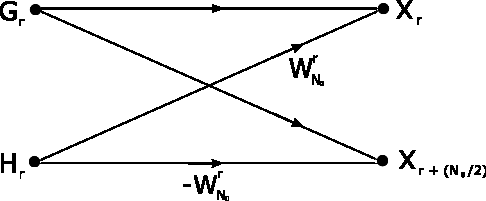
\includegraphics[width=0.5\linewidth]{Images/RevisaoDeLiteratura/Butterfly.pdf}
	\caption{Butterfly do Fluxo do Sinal}
	\vspace{-3.5mm}
	\caption*{Fonte: \citeonline[p.~721]{Lathi}}
	\label{fig:Butterfly}
\end{figure}
\vspace{4mm}

Aliando o conceito de divis�o em conquista ao m�todo de c�lculo da DFT, usando o diagrama \textit{Butterfly}, a representa��o do algoritmo da FFT pode ser facilmente representado pelo diagrama da Figura (\ref{fig:FFT8P}) \cite[p.~722]{Lathi}. Nesta figura, a FFT  � feita para apenas 8 amostras de sinal $X$.

\vspace{4mm}
\begin{figure}[H]
	\centering
	\captionsetup{width=1\textwidth, font=footnotesize, textfont=bf}	
	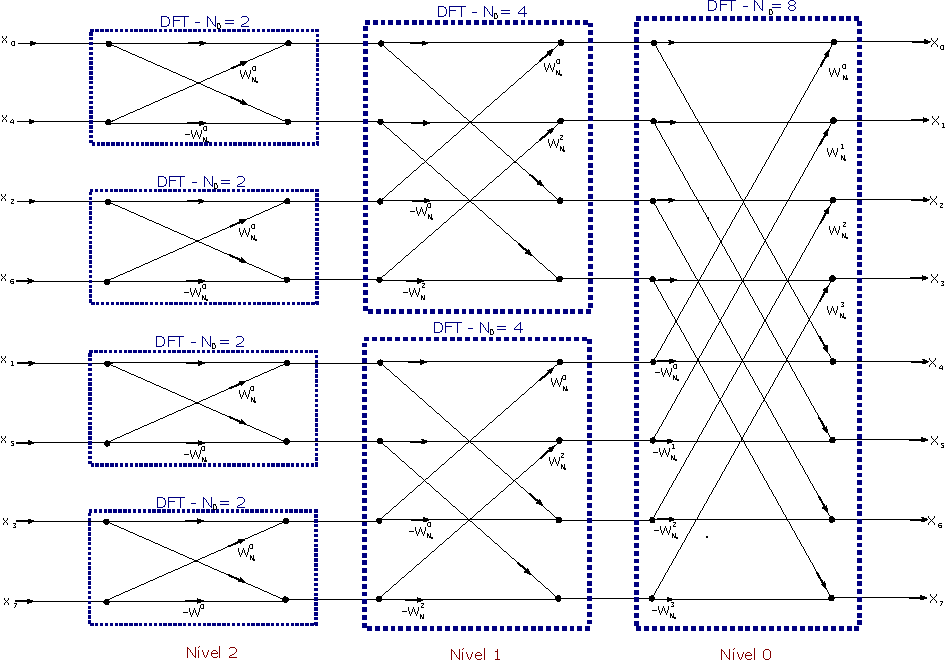
\includegraphics[width=1\linewidth]{Images/RevisaoDeLiteratura/FFT8P.pdf}
	\caption{FFT de 8 Pontos}
	\vspace{-3.5mm}
	\caption*{Fonte: \citeonline[p.~722]{Lathi}}
	\label{fig:FFT8P}
\end{figure}
\vspace{4mm}

Ap�s se dividir uma DFT de tamanho $N_0$ em duas DTFs de tamanho $N_0/2$,
e subdividindo cada uma das DFTs de tamanho $N_0/2$ em duas $N_0/4$ \cite[p.~721]{Lathi}. E assim o procedimento continua ate que se atinja um n�vel em que as DFTs tenham tamanho $N_0 / 2^n = 2$, ou seja, quando se atinge DFTs que possuam um custo de c�lculo m�nimo.

Um fato importante sobre o algoritmo da FFT � que o valor $N_0$ pode ser escolhido segundo a rela��o $N_0~=~r_n$, onde $n$ � o numero de n�veis necess�rios para calcular a FFT, e $r$ � o m�nimo tamanho DFT. Os algoritmos de FFT mais usados possuem a base $r$ igual a 2 ou a 4. Consequentemente, estes algoritmos s�o
conhecidos como Radix-2 e Radix-4, respectivamente \cite[p.~365]{Meyer}. Neste trabalho o foco ser� o algoritmo com a base $r$ igual a 2, ou seja, o Radix-2.

Na Figura (\ref{fig:FFT8P}) as DFTs est�o agrupadas por n�veis, onde cada n�vel abrange as DFTs de mesmo tamanho $N_0/n$, e no �ltimo n�vel a esquerda h� quatro DFTs de tamanho 2. O n�mero de n�veis necess�rios em uma FFT de $N_0$ pontos � $log_2 N_0$. Os valores de $X$, na Figura (\ref{fig:FFT8P})  � direita est�o ordenados de forma crescente, por�m os valores de $x$ � esquerda est�o ordenados de forma diferente. Est� ordena��o � conhecida como \textit{Bit-Reverse} \cite[p.~51]{Chu}.

Segundo \citeonline[p.~51]{Chu}, quando se divide o processo de c�lculo de uma DFT em duas, sendo uma respons�vel pelos valores pares e a outra pelo valores �mpares, conforme as conex�es entres o n�veis v�o ocorrendo, h� permuta��es entre os sinais. O processo de \textit{Bit-Reverse} prev� estas permuta��es, sendo poss�vel saber qual a ordem adequada dos sinais na entrada da FFT. Para aplicar o conceito de \textit{Bit-Reverse}, basta considerar um elemento $x_k$ de ordem $n$ e escrev�-lo na base binaria com $log_2 N_0$ bits. Em seguida, para determinar onde $x_k$ ser� ocupado, basta converter novamente para base decimal o n�mero bin�rio obtido, lendo esse na ordem inversa dos bits.

Na FFT da Figura (\ref{fig:FFT8P}) a subdivis�o das DFTs � deita a partir da sa�da, sinal em frequ�ncia, com DFT de 8 pontos, at� a entrada, sinal no tempo, com as DFTs de 2 pontos com custo m�nimo. Essa subdivis�o � conhecida como decima��o, e no caso da Figura (\ref{fig:FFT8P}), ela � feita a partir do sinal no tempo, logo essa estrutura � conhecida como Decima��o no Tempo. Por�m, existe uma outra forma, a decima��o na frequ�ncia. A partir de uma altera��o em (\ref{eq:DenicaoFFTA}), � poss�vel alterar a ordem da decima��o, partindo do sinal de entrada no tempo, at� a sa�da em frequ�ncia, como pode ser visto na Figura(\ref{fig:FFT8PDIF}) \cite[p.~37]{Chu}.

\vspace{4mm}
\begin{figure}[H]
	\centering
	\captionsetup{width=1\textwidth, font=footnotesize, textfont=bf}	
	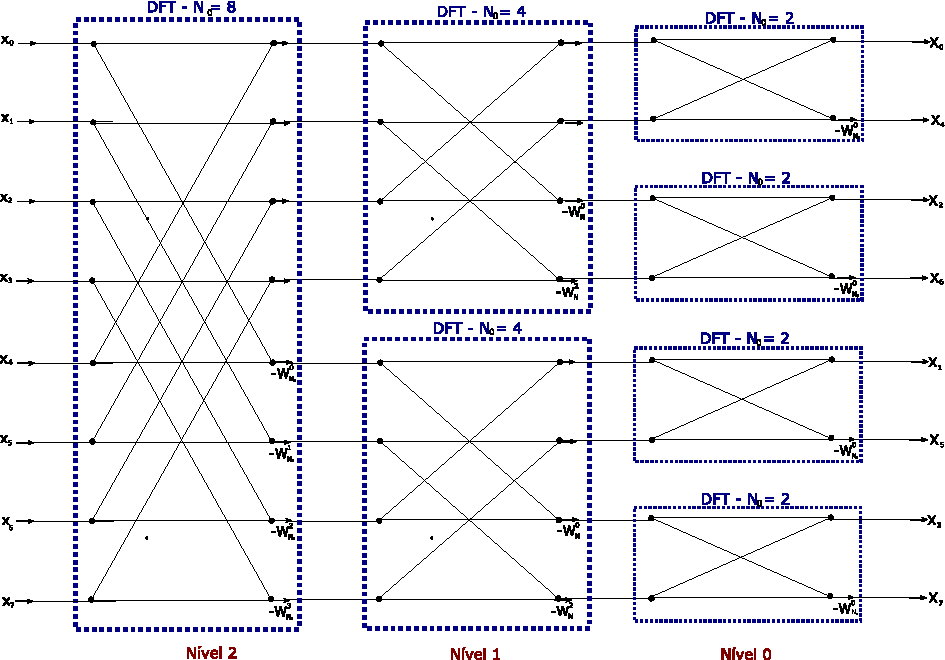
\includegraphics[width=1\linewidth]{Images/RevisaoDeLiteratura/FFT8PDIF.pdf}
	\caption{FFT DIF de 8 Pontos}
	\vspace{-3.5mm}
	\caption*{Fonte: Adaptado de \citeonline[p.~44]{Chu}}
	\label{fig:FFT8PDIF}
\end{figure}
\vspace{4mm}

Na decima��o em frequ�ncia, a ordem de entrada dos sinais na FFT ficar ordenados de forma crescente, por�m a sa�da passa a estar ordenado no esquema \textit{Bit-Reverse}. Este esquema de decima��o � preferencialmente escolhido por dispensar a reordena��o dos dados de entrada.

Ao final de todo o processo de simplifica��o do c�lculo da DFT, o algoritmo da FFT necessita apenas realizar $(N_0/2)~log_2~N_0$ multiplica��es e $N_0~log_2~N_0$ somas
complexas \cite[p.~720]{Lathi}. Desta forma, reduz-se assim a complexabilidade do
algoritmo, tornando a DFT pratic�vel at� para valores elevados de $N_0$.

	
\section{FPGA}
	Como afirma \citeonline[Pref�cio]{Meyer}, muitos algoritmos de processamento de sinais, como FFT \textit{(Fast Fourier Transform)} e os filtros FIR ou IIR, implementados anteriormente em PDSPs ou em Circuitos Integrados de Aplica��o Especifica ou ASIC \textit{(Application Specific Integrated Circuits)}, agora est�o sendo implementados em FPGAs.

\citeonline{moore}[p.~4] define a FPGA como um dispositivo semicondutor capaz de ser totalmente redefinido ap�s sua fabrica��o, permitindo ao desenvolvedor reconfigurar produtos e fun��es j� implementadas, adaptando o \textit{hardware} a novas fun��es. De forma pr�tica, a FPGA permite uma flexibilidade em um projeto, podendo mudar a forma como ele � implementado, sem a necessidade de se construir um \textit{hardware} novo.

\vspace{5mm}

	
\section{Algoritmo CORDIC}
	
\label{section:Cordic}
Na equa��o (\ref{eq:Xr}) nota-se que o c�lculo a FFT depende essencialmente de um multiplica��o complexa entre $W_{N_0}^r$ e $H_r$, onde $H_r$ representa um vetor complexo qualquer, e $W_{N_0}^r$ � igual a $e^{\frac{2\pi r}{N_0}}$. Esta tarefa pode ser realizada atrav�s da representa��o de $W_{N_0}^r$ e $H_r$ na forma retangular, considerando para efeitos de exemplo $W_{N_0}^r ~=~x+iy$ e $H_r~=~a+ib$, logo:

\begin{eqnarray}
	W_{N_0}^r ~=~x+iy, \\
	H_r~=~a+ib,\\
	H_r \cdot W_{N_0}^r~=~(x+iy)(a+ib), \\
	H_r \cdot W_{N_0}^r~=~(xa-yb)+i(xb+ya). 
\end{eqnarray}

Desta forma, ser�o necess�rios utilizar 4 multiplicadores e 2 somadores, para completar esta opera��o \cite[p.~1]{alvin}. Apesar disso, em termos de complexidade hardware, multiplicadores s�o mais elaborados e, em muitos dispositivos FPGA, possuem apenas algumas dezenas, o que limita a utiliza��o de multiplicadores em paralelo, reduzindo a velocidade de c�lculo da FFT.

Para contornar o problema, considere expressar o vetor $H_r$ na forma polar $re^{\theta_r}$ e manter $W_{N_0}^r$ igual a $e^{\frac{2\pi r}{N_0}}$, logo:

\begin{eqnarray}
	H_r~=~Re^{\left(\theta_r\right)}, \\
	H_r \cdot W_{N_0}^r~=~re^{\left(\theta_r\right)} \cdot e^{\left(\frac{2\pi r}{N_0}\right)}, \\
	H_r \cdot W_{N_0}^r~=re^{\left(\theta_r+\frac{2\pi r}{N_0}\right)}.
\end{eqnarray}

Assim $H_r \cdot W_{N_0}^r$ � equivalente a opera��o trigonom�trica de rotacionar o vetor complexo $H_r$ pelo �ngulo de $2\pi r/N_0$, como pode ser visto na Figura (\ref{fig:RotacaoVetorA0}).

\vspace{6mm}
\begin{figure}[H]
	\centering
	\captionsetup{width=0.5\textwidth, font=footnotesize, textfont=bf}	
	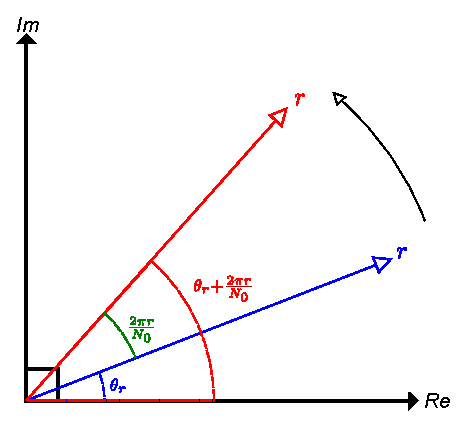
\includegraphics[width=0.5\linewidth]{Images/RevisaoDeLiteratura/RotacaoVetorA0.eps}
	\caption{Rota��o de $H_r$ pelo �ngulo de $2\pi r/N_0$}
	\vspace{-3.5mm}
	\caption*{Fonte: Autoria Pr�pria}
	\label{fig:RotacaoVetorA0}
\end{figure}
\vspace{6mm}

Implementar opera��es trigonom�tricas sem utilizar multiplicadores, para evitar o gargalo que eles possam provocar, parece dif�cil, por�m existe uma t�cnica bastante usada no desenvolvimento de circuitos l�gicos em FPGA que o possibilita. Com o objetivo de oferecer uma solu��o para o c�lculo de fun��es trigonom�tricas mais simples, utilizando o m�nimo de recursos de tempo e \textit{hardware}, Jack E. Volder\cite{Volder} desenvolveu a t�cnica de computa��o trigonom�trica CORDIC (\textit{COordinate Rotation DIgital Computer}).


\subsection{CORDIC Tradicional}
\label{sec:CoricTradicional}

O algoritmo CORDIC tem como base as micro-rota��es do vetor alvo, de tal modo que cada micro-rota��o possa ser feita por somas e deslocamentos de bits. Para tal, considere o vetor $H_r ~ = ~x~+~iy$, e a matriz de rota��o $A$ em fun��o do angulo $\theta$. A rota��o do vetor pode ser dada por \cite{Garrido}:

\begin{equation}
	\left[\begin{array}{c}
	x' \\ 
	y' \\ 
	\end{array}\right] = \left[\begin{array}{cc}
	cos(\theta) & -sin(\theta)\\ 
	sin(\theta) & cos(\theta) \\ 
	\end{array}\right] \left[\begin{array}{c}
	x \\ 
	y \\ 
	\end{array}\right].
	\label{eq:rotacaoVetorial}
\end{equation}
   
  
Isolando o termo $cos( \theta )$ de (\ref{eq:rotacaoVetorial}) � obtido o seguinte sistema:

\begin{equation}
	\left[\begin{array}{c}
	x' \\ 
	y' \\ 
	\end{array}\right] = cos(\theta) \left[\begin{array}{cc}
	1 & -tan(\theta)\\ 
	tan(\theta) & 1 \\ 
	\end{array}\right] \left[\begin{array}{c}
	x \\ 
	y \\ 
	\end{array}\right],
	\label{eq:rotacaoVetorialB}
\end{equation}

o qual � a base da t�cnica CORDIC convencional \cite{Motaz}.

Segundo \cite{Volder}, ao inv�s de rotacionar completamente o vetor $H_r$ pelo �ngulo $\theta$, ou pelo �ngulo $2\pi r/N_0$ como  mostrado na Figura (\ref{fig:RotacaoVetorA0}),  o algoritmo CORDIC rotaciona $H_r$ por �ngulos $\theta_n$ muito menores, sendo estes fra��es de $\theta$, de tal forma que:

\begin{equation}
	\theta ~=~ \sum_{n = 0}^{N-1} \mu_n \theta_n + \zeta,
	\label{eq:aproximation}
\end{equation}

onde e $\mu_n$ representa o sentido da micro rota��o $\theta_n$, sendo que se for no sentido hor�rio � igual a 1, caso contr�rio � igual a -1, e $\zeta$ � o erro acumulado da aproxima��o pelo somat�rio, que ser� considerado suficientemente pequeno para ser ignorado. 

O primeiro ponto dessa abordagem � o fato de que se um angulo $\theta_n$ for suficientemente pequeno � poss�vel afirmar que:

\begin{equation}
	\theta_n~\simeq~tan^{-1} \theta_n.
	\label{eq:AproximacaoThetaTan}
\end{equation}
 
Assim � poss�vel substituir $\theta$ no sistema de (\ref{eq:rotacaoVetorialB}), e  obter a seguinte express�o:

\begin{equation}
	\left[\begin{array}{c}
	x' \\ 
	y' \\ 
	\end{array}\right] = cos(tan^{-1} \theta_n) \left[\begin{array}{cc}
	1 & -tan(tan^{-1} \theta_n)\\ 
	tan(tan^{-1} \theta_n) & 1 \\ 
	\end{array}\right] \left[\begin{array}{c}
	x \\ 
	y \\ 
	\end{array}\right].
	\label{eq:rotacaoVetorialC}
\end{equation}

O segundo ponto � que para satisfazer (\ref{eq:aproximation}) s� � necess�rio que a soma do conjunto de micro rota��es $\theta_n$ resulte no �ngulo $\theta$, o que abre a possibilidade de se escolher um conjunto de micro rota��es baseadas em deslocamento de bits, como:

\begin{equation}
	\theta_n ~=~ tan^{-1} 2^{-n}
	\label{eq:EquivalenciaThetaTan}
\end{equation}

Logo, aplicando a Equa��o(\ref{eq:EquivalenciaThetaTan}) em (\ref{eq:rotacaoVetorialC}), � obtido a express�o final para CORDIC:

\begin{equation}
	\left[\begin{array}{c}
	x' \\ 
	y' \\ 
	\end{array}\right] = \prod_{n=0}^{N-1} K_c \left[\begin{array}{cc}
	1 & -\mu 2^{-n}\\ 
	\mu 2^{-n} & 1 \\ 
	\end{array}\right] \left[\begin{array}{c}
	x \\ 
	y \\ 
	\end{array}\right],
	\label{eq:rotacaoVetorialD}
\end{equation}

\begin{equation}
	k_c = cos(tan^{-1} (2^{-n})) = \frac{1}{\sqrt{1 + 2^{-2n}}},
	\label{eq:K}
\end{equation}

onde:

\begin{equation}
	\mu \in \{-1,1\} 
\end{equation}

$K_c$  � calculado a cada micro-rota��o $n$, assim seu valor total � dado pelo produto de todos os $N$ ganhos.  O n�mero total de micro-rota��es ($N$) � escolhido de acordo com o SQNR  (\textit{Signal-to-Quantization-Noise Ratio }) admiss�vel a cada rota��o. Segundo \cite{Volder}, considerando $N\rightarrow\infty$, $K_c$ � passa a ser constate e aproximadamente igual a $0,6073$. O inverso de $K_c$ � igual a $1,647$, sendo conhecido como Ganho CORDIC. Tal ganho � independe do �ngulo a ser rotacionado, e em muitos sistemas este ganho � s� compensado fora do bloco l�gico de c�lculo do CORDIC.

Como pode ser observado, o algoritmo CORDIC se resume a opera��es de deslocamento de \textit{bit} e somas. A dire��o das micro-rota��es � determinada por $\mu$, que depende diretamente do sinal do �ngulo $\theta_n$ a se rotacionar. Em aplica��es onde o �ngulo a se rotacionar � previamente conhecido, que � o caso da FFT,  as sequ�ncias de rota��es $\mu$ podem ser armazenado em uma mem�ria  \sigla[Read-Only Memory]{ROM} \cite{Motaz} \textit{Read-Only Memory}. Isto torna as micro-rota��es como $n$ intera��es, armazenando em $z$ os �ngulos rotacionados a cada intera��o de $\theta_n$, sendo o algoritmo CORDIC expressado por:

\begin{eqnarray}
	x(n+1) = x(n) - [\mu 2^{-n}]y(n), \\
	y(n+1) = y(n) + [\mu 2^{-n}]x(n), \\
	z(n+1) = z(n)-tan^{-1} [\mu 2^{-n}], \\
	\label{eq:CORDIC}
\end{eqnarray}

onde:

\begin{eqnarray}
	H_r~=~x(0)+iy(0),\\
	\theta ~=~z(0), \\
	n~=~\left\{0, 1, ..., N-1\right\}, \\
	\mu~=
	\begin{bmatrix}
		1 & z \left(n \right) \geq 0, \\
		-1 & z \left(n \right) < 0 
	\end{bmatrix}.
	\label{eq:CORDICRules}
\end{eqnarray}


\subsection{EEAS-CORDIC}

No algoritmo CORDIC, cada �ngulo de rota��o $\theta_n$ � necessariamente determinado de maneira sequencial ap�s cada intera��o $n$, utilizando o conjunto de �ngulos elementares definidos como \cite{Cheng}:

\begin{eqnarray}
	S_1 = \{ tan^{-1} ( \mu 2^{-n} ) \}, \\
	:~\mu \in \{-1,1\},~n\in \{0,1, \dots, N-1\}.
	\label{eq:s0}
\end{eqnarray}

A partir do �ngulo inicial de $H_r$, o algoritmo Cordic realiza as $N$ intera��es, deslocando o vetor por meio do conjunto de �ngulos elementares, de forma a reduzir a diferen�a entre o �ngulo atual e o �ngulo desejado. Para fins de compara��o a  Figura (\ref{fig:CordicComparationCordic}) apresenta a densidade combinacional dentro do circulo unit�rio do conjunto de �ngulos elementares do algoritmo CORDIC tradicional.

\vspace{5mm}
\begin{figure}[H]
	\centering
	\captionsetup{width=0.6\textwidth, font=footnotesize, textfont=bf}	
	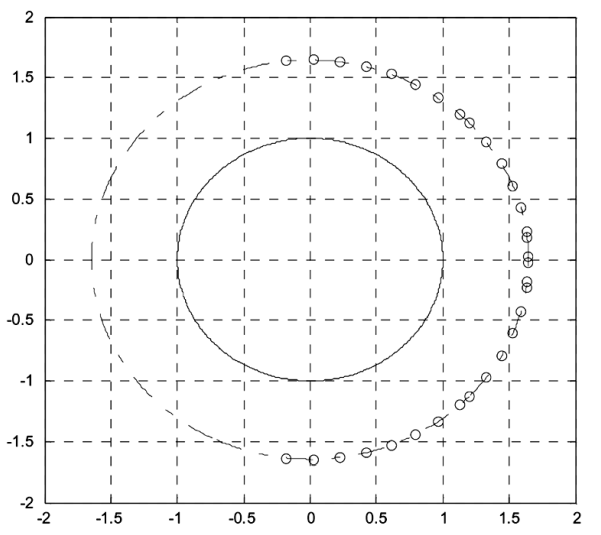
\includegraphics[width=0.6\linewidth]{Images/RevisaoDeLiteratura/CordicComparationCordic.PNG}
	\caption{�ngulos Elementares - Cordic Tradicional com N=4}
	\vspace{-3.5mm}
	\caption*{Fonte: \cite{Chih}}
	\label{fig:CordicComparationCordic}
\end{figure} 
\vspace{5mm}

Segundo \citeonline{Shing} o maior problema do CORDIC � a baixa velocidade computacional de c�lculo deste algoritmo, devido principalmente a necessidade de um grade  n�mero de intera��es $N$ para atingir um erro de aproxima��o $\zeta$ aceit�vel. O error de aproxima��o $\zeta$ � dado por:

\begin{equation}
	\zeta = \left| \theta~-~\sum_{n=0}^{N-1} \mu \theta_n \right| ~ =~ \left| \theta~-~\sum_{n=0}^{N-1}  \mu ~ tan^{-1} (2^{-n}) \right|,
	\label{eq:erroTheta}
\end{equation} 
onde:

\begin{equation}
\mu \in \{-1,~0,~1\}
\end{equation} 

Em aplica��es onde os �ngulos de rota��o s�o conhecidos, � poss�vel relaxar as restri��es da Equa��o (\ref{fig:CordicComparationCordic}), utilizando o m�todo \textit{Angle Recoding} (AR) \cite{Shing}. Os AR tem como objetivo reduzir o n�mero de intera��es CORDIC e  o erro $~\zeta~$. Para tal, o AR que expande o conjunto de combina��es lineares em (\ref{eq:s0}), adicionando zero ao conjunto de $\mu$. Com isso, obt�m-se uma melhor aproxima��o para certos valores de $\theta$ e uma redu��o de at� 50\% no n�mero de intera��es \cite{Meher}. 

Por outro lado, o m�todo \textit{Extended Elementary-Angle-Set Recoding} (EEASR) apresenta um m�todo baseado no AR que, al�m de expandir o conjunto de $\mu$, estende tamb�m o conjunto de �ngulos elementares (\textit{Elementary-Angle-Set}, EAS), visando aumentar a possibilidades de decomposi��o do �ngulo de rota��o\cite{Cheng}. Para perceber a modifica��o que o EEASR prop�em, nota-se primeiramente que o conjunto de �ngulos elementares no CORDIC utilizando AR � definido como:

\begin{eqnarray}
	S_1 = \{ tan^{-1} ( \mu 2^{-s} ) \}, \\
	:~\mu \in \{-1,0,1\},~s\in \{0,1, \dots, N-1\}. 
	\label{eq:s1}
 \end{eqnarray}    
 
Como � poss�vel notar em (\ref{eq:s1}), os �ngulos elementares dependem de apenas um termo pot�ncia de dois, ou \textit{Signed Power of Two} (SPT). Segundo \cite{Cheng}, para aumentar a precis�o dos �ngulos elementares e, consequentemente, reduzir o n�mero de intera��es pode-se adicionar mais um termo SPT em  (\ref{eq:s1}). 

Assim:
  
\begin{eqnarray}
	 S_2 = \{ tan^{-1} ( \mu_{0} 2^{-s_0} + \mu_{1} 2^{-s_1}) \} \\ 
    :~\mu_{0},\mu_{1} \in \{-1,0,1\},~s_0,s_1 \in \{0,1, \dots, S\} 
    \label{eq:S2}
\end{eqnarray} 

onde $S$ � denominado como o n�mero m�ximo de deslocamentos de \textit{bits} a direita que podem ser realizados. Este valor est� diretamente relacionado com o quantidade de \textit{bits} utilizados para representar um n�mero dentro da arquitetura onde o CORDIC � implementado. Por exemplo, em uma aplica��o em FPGA, onde a palavra bin�ria utilizada para representar um n�mero inteiro tenha apenas 16 \textit{bits}, n�o faz sentido o valor de $S$ ser maior do 15. Portanto, alterando a equa��o (\ref{eq:rotacaoVetorialC}) com base em  (\ref{eq:S2}) � obtido a express�o para c�lculo interativo CORDIC utilizando o EEASR:


\begin{eqnarray}
	\left[\begin{array}{c}
	x(n+1) \\
	y(n+1) \\
	\end{array}\right]
	\left[\begin{array}{cc}
	1 & \mu_{0}2^{-s_0 (n)} + \mu_{1}2^{-s_1 (n)} \\
	\mu_{0}2^{-s_0 (n)} + \mu_{1}2^{-s_1 (n)} & 1 \\
	\end{array}\right] \left[\begin{array}{c}
	x(n) \\
	y(n) \\
	\end{array}	\right],\\
	:~\mu_{i},\mu_{j} \in \{-1,0,1\},~s_0,s_1 \in \{0,1, \dots, S\},
	\label{eq:EEASR}
\end{eqnarray}

\begin{equation}
	\theta_n~=~tan^{-1} \left(\mu_{0}2^{-s_0 (n)} + \mu_{1}2^{-s_1 (n)} \right)
	\label{eq:EEASRtheta},
\end{equation}

\begin{equation}
	z(n+1)~=~z(n-1)+\theta_n,
	\label{eq:EEASRSync}
\end{equation}


� importante notar que ao adicionar mais termos a $S_1$, o ganho $K_c$ tamb�m � modificado, passando a ser definido por:

\begin{equation}
	K_n~=~\frac{1}{\sqrt{1+ [\mu_{0}2^{-s_0 (n)} + \mu_{1}2^{-s_1 (n)}]^2}}.
	\label{eq:EEASRKcn}
\end{equation}

Com a altera��o de $K_c$, o ganho passa a n�o ser mais constante, e varia de acordo com cada intera��o $N$. Sendo assim necess�rio calcular o ganho $K_c$ para cada intera��o afim de realizar a compensa��o. O valor de $K_c$ ao final de cada opera��o de c�lculo CORDIC passa a ser definido por: 

\begin{equation}
	K_c~=~\prod_{n=0}^{N-1} K_n.
	\label{eq:EEASRKc}
\end{equation}

Para casos em que o �ngulo $\theta$ a ser rotacionado � conhecido, como � o caso da FFT, � poss�vel escolher previamente o conjunto de valores $\mu_{0}$, $\mu_{1}$, $s_{0}$ e $s_{1}$, e consequentemente atrav�s da Equa��o (\ref{eq:EEASRKcn}) determinar o valor de $K_c$ a ser compensado a cada intera��o, e por meio de  (\ref{eq:EEASRKc}) determinar a compensa��o de $K_c$ a ser realizada ap�s cada opera��o de rota��o. Para tal � realizado, ap�s as intera��es de rota��o do algoritmo, uma corre��o no m�dulo do vetor resultante por meio da seguinte opera��o de rota��o modificada:

\begin{eqnarray}
	x(n+1) = x(n) - [\mu_{0}2^{-s_0 (n)} + \mu_{1}2^{-s_1 (n)}]x(n), \\
	y(n+1) = y(n) - [\mu_{0}2^{-s_0 (n)} + \mu_{1}2^{-s_1 (n)}]y(n), \\
	z(n+1) = z(n).
	\label{eq:EEASRKcCorrection}
\end{eqnarray}

onde $\mu_{0}$, $\mu_{1}$, $s_{0}$ e $s_{1}$ para esta opera��o s�o escolhidos de modo a minimizar o erro de compensa��o de $K_c$. 

Com a relaxa��o das restri��es introduzidas pelo m�todo AR e pelo EEASR, a densidade combinacional dentro do circulo unit�rio do conjunto de �ngulos elementares do Algoritmo CORDIC aumenta, se comparado ao CORDIC tradicional, como pode ser visto na Figura (\ref{fig:CordicComparationEEAS}). 

\vspace{5mm}
\begin{figure}[H]
	\centering
	\captionsetup{width=0.6\textwidth, font=footnotesize, textfont=bf}	
	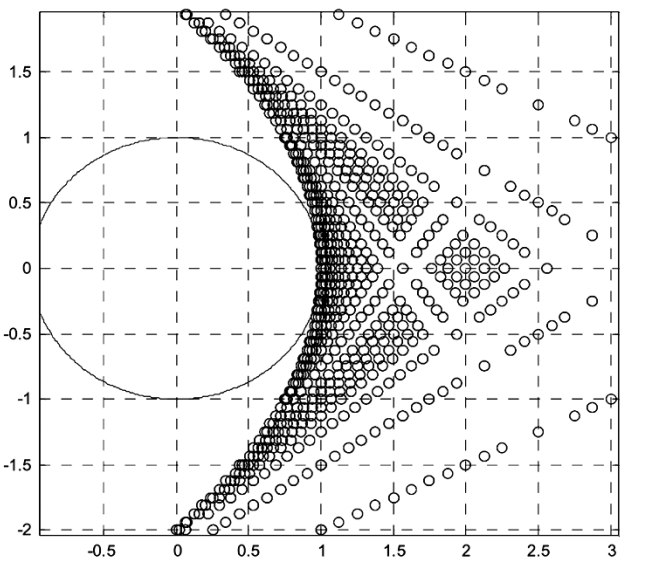
\includegraphics[width=0.6\linewidth]{Images/RevisaoDeLiteratura/CordicComparationEEAS.PNG}
	\caption{EEAS com N=2 e S=4}
	\vspace{-3.5mm}
	\caption*{Fonte: \citeonline{Chih}}
	\label{fig:CordicComparationEEAS}
\end{figure}    
\vspace{5mm}

\subsubsection{Algoritmo TBS}
\label{section:TBS}

A relaxa��o das restri��es feita pelos m�todos AR e  EEASR tornaram o algoritmo iterativo CORDIC mais eficiente, por�m ele abre uma quest�o crucial: a determina��o dos conjuntos $\mu$ e $s$. No algoritmo CORDIC tradicional, o valor de $\mu$ estava contido no conjunto $\{-1, 1\}$ e era determinado com base no sinal de $z(n)$ a cada intera��o. No entanto, no m�todo AR $\mu$ passa a estar contido no conjunto $\{-1, 0, 1\}$. Logo, determinar o valor de $\mu$ a cada intera��o torna-se uma tarefa de otimiza��o, em rela��o a minimizar o erro $\zeta$, na forma \cite{Cheng}:

\begin{equation}
	min~\zeta~=~\left| \theta~-~\sum_{n=0}^{N-1}  \mu ~ tan^{-1} (2^{-n}) \right|,
	\label{eq:MinZeta}
\end{equation} 

onde:

\begin{equation}
	\mu \in \{-1,~0,~1\}.
\end{equation} 

No algoritmo CORDIC convencional o conjunto dos �ngulos elementares � definido por $S_1$ em (\ref{eq:s0}), e a cada intera��o o deslocamento do vetor � feito com base  no elemento $n$ deste conjunto. O m�todo EEASR adiciona mais um termo SPT a express�o do conjunto dos �ngulos elementares $S_2$, definido em (\ref{eq:S2}), o que possibilita a escolha de qualquer termo $s_0$ e $s_1$. Desta forma, al�m de agregar a mesma necessidade de determinar o conjunto otimizado $\mu_0$ e $\mu_1$ de AR, o EEASR tamb�m requer a determina��o do conjunto otimizado $s_0$ e $s_1$, visando minimizar tamb�m o erro $\zeta$. Portanto, a fun��o de minimiza��o do erro $\epsilon$ � dada pela seguinte express�o: 

\begin{eqnarray}
	min~\zeta~=~\left| \theta~-~\sum_{n=0}^{N-1}  tan^{-1} (\mu_{0} 2^{-s_0} + \mu_{1} 2^{-s_1}) \right|, \\
	:~\mu_{0},\mu_{1} \in \{-1,0,1\},~s_0,s_1 \in \{0,1, \dots, S\}.
	\label{eq:MinZeta0}
\end{eqnarray} 

Para otimizar a Fun��o (\ref{eq:MinZeta0})  � poss�vel utilizar um variedade de algoritmos heur�sticos ou n�o heur�stico a fim de determinar um conjunto de par�metros que minimize o erro $\zeta$, como por exemplo \textit{Dijkstra}, Caminhos M�nimos ou o mais comum Algoritmo \textit{Greedy}. \citeonline{Cheng} prop�e um m�todo de otimiza��o para par�metros EEAS chamado \textit{Trellis-Based Search}(TBS). 

A partir do n�mero m�ximo de intera��es $N$, do �ngulo de rota��o $\theta$ e de $W$, que representa numero de bits de $\theta$, o TBS emprega um m�todo de otimiza��o para encontrar os melhores par�metros $s^0(n)$, $s^1(n)$, $\mu_{0}$ e $\mu_{1}$ \cite{Cheng}. \textit{TBS} � baseado no efeito que os diferentes arranjos dos �ngulos elementares $S_2$ poss�veis tem sobre $\zeta$. O algoritmo segue o seguintes passos:

\begin{enumerate}
	\item \textit{Inicializa��o:} Inicialmente � definido o vetor $r(k)$, o qual representa o conjunto de �ngulos elementares presentes na Equa��o  (\ref{eq:MinZeta0}), obtidos atrav�s das poss�veis combina��o n�o redundantes de $\mu_{0}$, $\mu_{1}$, $s_0$ e $s_1$. Em seguida, � definido a matriz $\phi(n,k)$ para ($1 \leq n \leq N$)  e ($1 \leq k \leq z(S_2)$), representando a estrutura de acumula��o do algoritmo utilizada para alcan�ar o melhor resultado.  $N$ � o n�mero de intera��es desejadas, enquanto $z(S_2)$ representa o n�mero de elementos do vetor $r(k)$. Para ent�o iniciar o algoritmo, $\phi(1,k)$ � preenchido com o vetor $r(k)$.
	
	\item \textit{Acumula��o:} Em cada itera��o $n$ o algoritmo percorre os elementos $k$ do vetor $\phi(n+1,k^*)$, atribuindo a cada valor $k$  o menor resultado encontrado da express�o $\| \phi(n,k^*) + r(k) - \theta \|$. O �ndice $i$ varia $1 \leq i \leq N-1$, e $k$ varia de $1 \leq k \leq Z(S_2)$. 
	
	\item \textit{Determina��o do �timo Global:} Ao final do processo de acumula��o, os elemento da coluna $\phi(N,)$ apresentam os resultados globais. Logo, dentro desta coluna � determinado o valor que mais se aproxima de $\theta$, defini-se este como $\theta_{TBS}$.
	
	\item \textit{Determina��o do Caminho Solu��o:} A partir do elemento $\theta_{TBS}$ da coluna $\phi(N,)$ � tra�ado o caminho reverso at� a coluna $\phi(1,)$. A come�ar por $(k'=\theta_{TBS})$ e $(i=N)$ �  escolhido o valor da coluna $(i-1)$ que minimiza $\| \phi(1:z(S_2),i-1) + r(k') - \theta \|$. Em seguida se atribui a $k'$ a posi��o $k$ do valor minimizante. Os valores $k'$ s�o armazenados em um vetor e representam as combina��es de �ngulos elementares que minimizam o erro $\epsilon$.
\end{enumerate}

Segue abaixo o pseudo-c�digo que implementa o algoritmo TBS.
 
\vspace{3mm}
\lstset{style=VHDL}
	\begin{lstlisting}[caption={Algoritmo TBS \\ Fonte : \citeonline{Cheng}},captionpos=b, mathescape]
		% Inicializa��o
		$\displaystyle \phi(1,k)~=~r(k)$ para todo k,
		
		%Acumula��o
		$\displaystyle FOR~i=1~to~N-1$
			$\displaystyle FOR~k=1~to~Z(S_2)$
				$\displaystyle \phi(i+1, k) ~=~ min \left\{ \mid \phi(i,k^*)+r(k)-\theta \mid : 1 \leq k^* \leq Z(S_2) \right\}$
			$\displaystyle END$
		$\displaystyle END$
		
		%Determina��o do �timo Global
		$\displaystyle \theta_{TBS}~=~min \left\{ \mid \phi(R_m,k^*)-\theta \mid : 1 \leq k^* \leq Z(S_2) \right\}$
		$\displaystyle Result(N)~=~k^*$
		
		%Determina��o do Caminho Solu��o
		$\displaystyle FOR~i=N~to~2$
			$\displaystyle Encontra~k'~tal~que~\phi(i,k^*)~=~min \left\{ \mid \phi(i-1,k')+r(k^*)-\theta \mid : 1 \leq k' \leq Z(S_2) \right\}$
			$\displaystyle k^*=k'$
			$\displaystyle Result(i-1)=k'$
		$\displaystyle END$
	\end{lstlisting}
	\label{code:PCTBS}
\vspace{3mm}


Nos trabalhos de  \citeonline{Cheng}, os autores utilizam um exemplo base para explicar o algoritmo TBS, o qual tamb�m ser� usado aqui. Para este exemplo, o �ngulo de rota��o $\theta$ ser� $pi/3$, o n�mero m�ximo de intera��es ser� $N=4$ e a resolu��o de $\theta$ ser� de $W=~4$ bits. 


A primeira etapa do algoritmo ent�o inicia com a defini��o do vetor $r(k)$, e o preenchimento da primeira coluna da matriz $\phi(1, )$, como pode ser visto na Figura (\ref{fig:TBSExempleA}). Na segunda etapa do algoritmo � realizada a acumula��o, onde cada elemento das colunas 2, 3 e 4 s�o preenchidos com base na coluna anterior a partir da express�o $\| \phi(n,k^*) + r(k) - \theta \|$. Na Figura (\ref{fig:TBSExempleA}) o elemento $\phi(2,15) $ representa esta etapa, onde o valor do elemento $\phi(2,15)$ � definido a partir da soma do �ngulo representante da linha 15 (r(15)), com o elemento da coluna 1 que minimiza o erro de aproxima��o do resultado desta soma com $\theta$, que neste caso � $\pi/3$. Este processo se estende at� completar a coluna 4 da matriz $\phi$.

\vspace{5mm}
\begin{figure}[H]
	\centering
	\captionsetup{width=0.6\textwidth, font=footnotesize, textfont=bf}	
	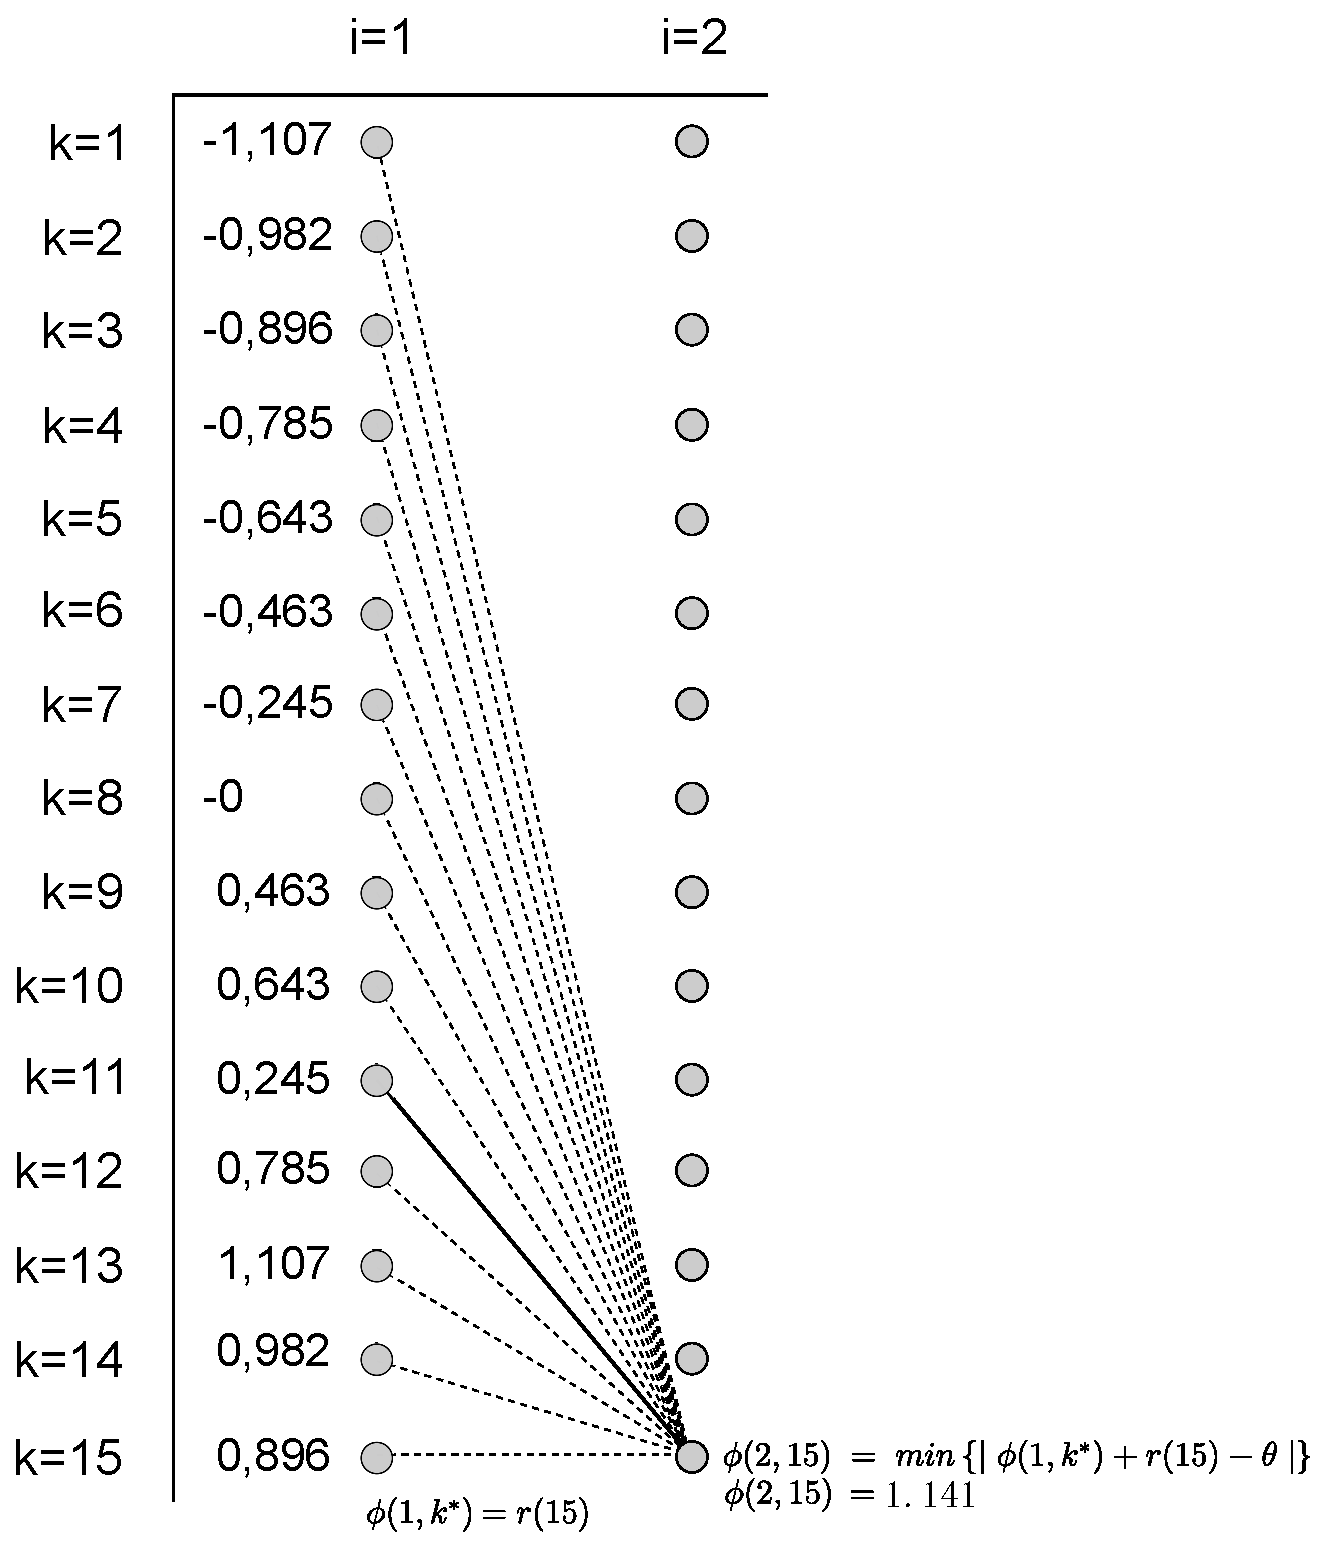
\includegraphics[width=0.6\linewidth]{Images/RevisaoDeLiteratura/TBSExempleA.eps}
	\caption{Exemplo de execu��o do Algoritmo TBS}
	\vspace{-3.5mm}
	\caption*{Fonte: Autoria Pr�pria}
	\label{fig:TBSExempleA}
\end{figure}    
\vspace{5mm}

Ap�s a etapa de acumula��o, a �ltima coluna de $\phi$ apresenta os resultados globais da acumula��o. Logo, para determinar o valor �timo global � escolhido na coluna  $\phi(4,)$ o valor $\theta_{TBS}$, que mais se aproxima de $\theta$ ou $\pi/3$. Ap�s esta etapa  � iniciada a determina��o do vetor $Result$, o qual deve conter o caminho solu��o necess�rio para atingir o valor de �timo global $\theta_{TBS}$. Na Figura (\ref{fig:TBSExempleB}) � apresentado os caminhos m�nimos para cada coluna da matriz  $\phi$, consequentemente, o melhor caminho encontrado pelo algoritmo.

\vspace{5mm}
\begin{figure}[H]
	\centering
	\captionsetup{width=0.6\textwidth, font=footnotesize, textfont=bf}	
	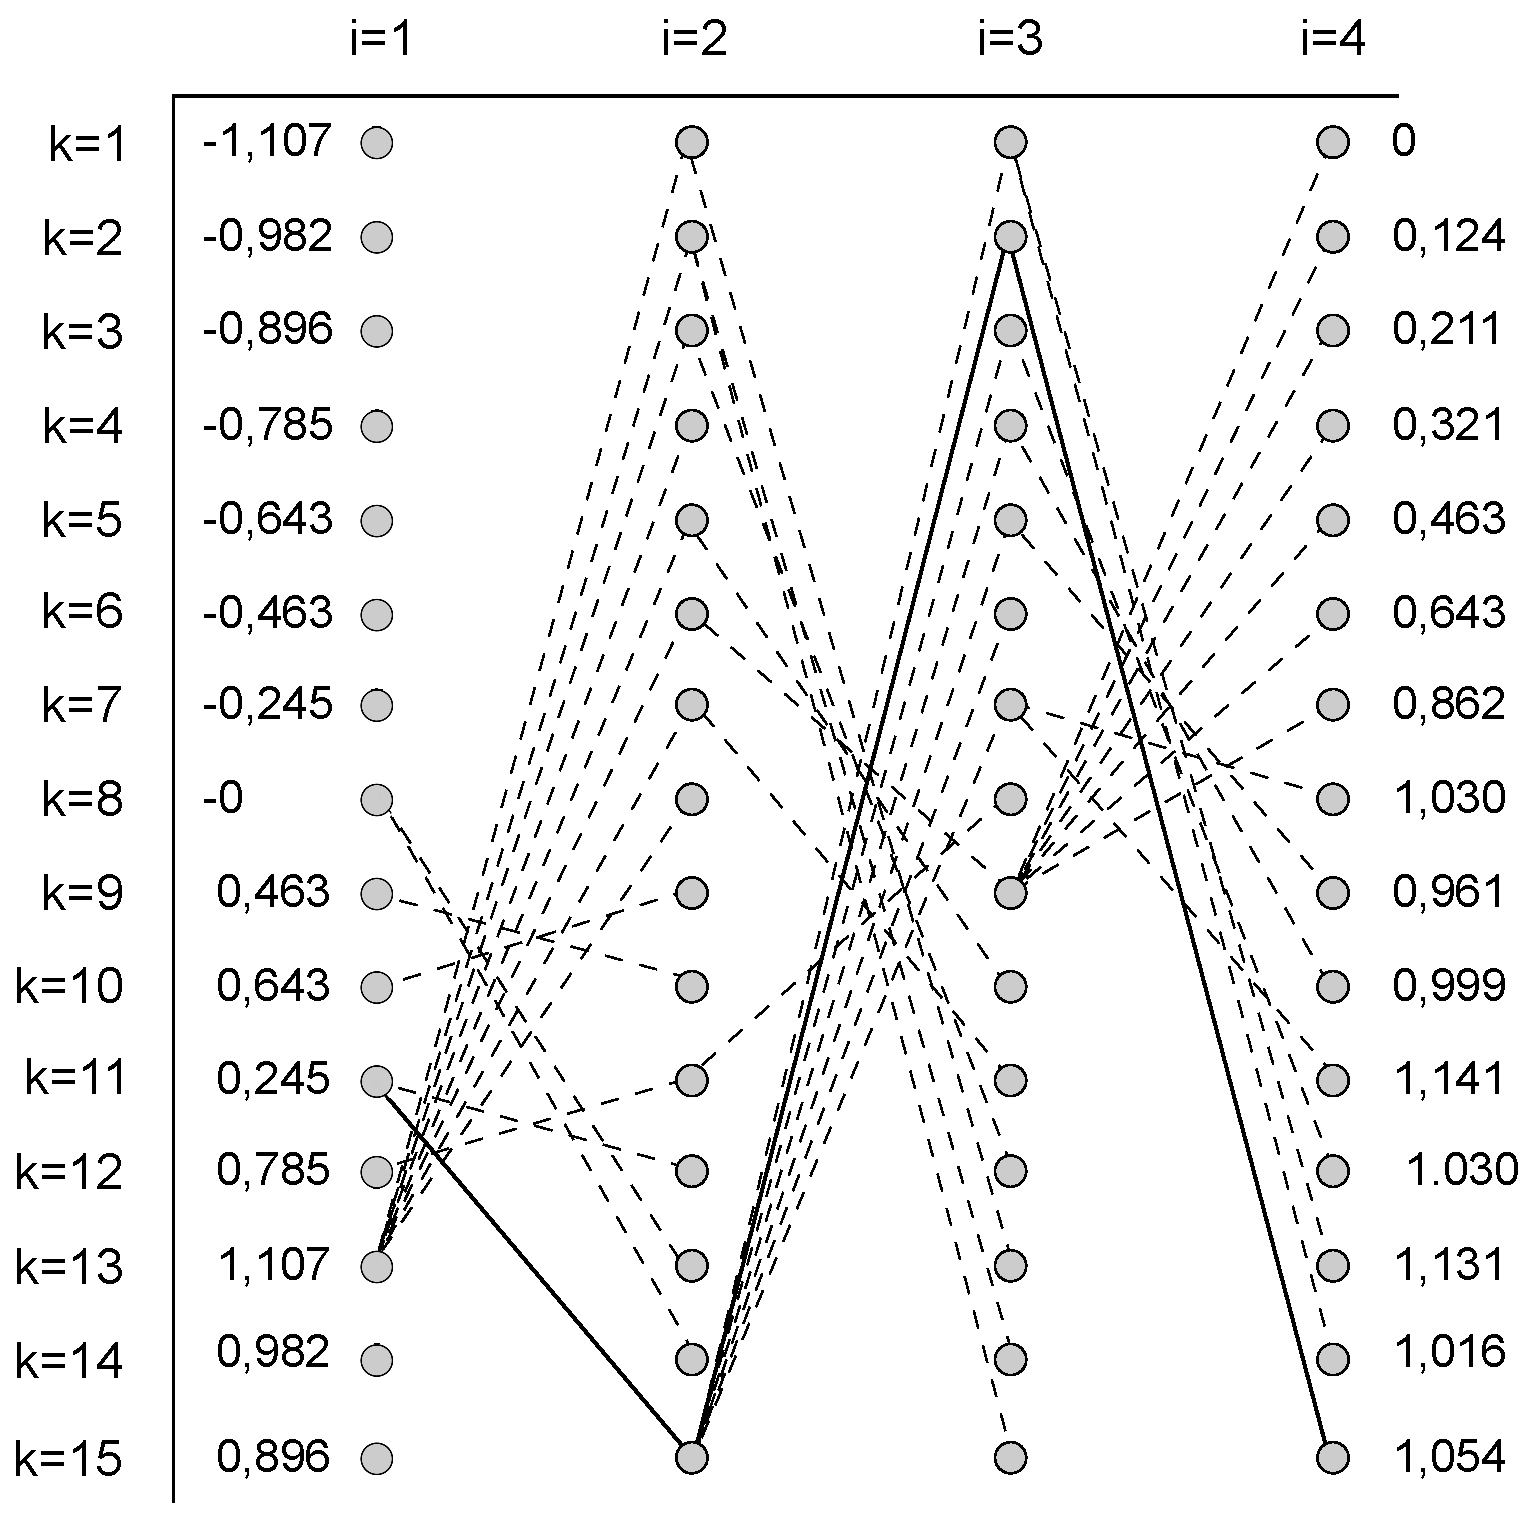
\includegraphics[width=0.6\linewidth]{Images/RevisaoDeLiteratura/TBSExempleB.eps}
	\caption{Exemplo de execu��o do Algoritmo TBS}
	\vspace{-3.5mm}
	\caption*{Fonte: Autoria Pr�pria}
	\label{fig:TBSExempleB}
\end{figure}    
\vspace{5mm}

A tabela (\ref{tab:TBSExemple}) apresenta os valores encontrados para $\phi$ na execu��o do exemplo apresentado. Em destaque est�o os valores do caminho solu��o,  que s�o armazenados em $Result$.

\vspace{5mm}
\begin{table}[h]
	\centering
	\captionsetup{width=.5\linewidth}
	\begin{tabular}{c|c|c|c|c|}
		\cline{2-5}
		& \cellcolor[HTML]{333333}{\color[HTML]{FFFFFF} i=1} & \cellcolor[HTML]{333333}{\color[HTML]{FFFFFF} i=2} & \cellcolor[HTML]{333333}{\color[HTML]{FFFFFF} i=3} & \cellcolor[HTML]{333333}{\color[HTML]{FFFFFF} i=4} \\ \hline
		\multicolumn{1}{|c|}{\cellcolor[HTML]{333333}{\color[HTML]{FFFFFF} k=1}}  & -1.1071                                            & 0                                                  & 0.0339                                             & 0                                                  \\ \hline
		\multicolumn{1}{|c|}{\cellcolor[HTML]{333333}{\color[HTML]{FFFFFF} k=2}}  & -0.9828                                            & 0.1244                                             & \cellcolor[HTML]{FD6864}0.1582                     & 0.1244                                             \\ \hline
		\multicolumn{1}{|c|}{\cellcolor[HTML]{333333}{\color[HTML]{FFFFFF} k=3}}  & -0.8961                                            & 0.2111                                             & 0.2450                                             & 0.2111                                             \\ \hline
		\multicolumn{1}{|c|}{\cellcolor[HTML]{333333}{\color[HTML]{FFFFFF} k=4}}  & -0.7854                                            & 0.3218                                             & 0.3556                                             & 0.3218                                             \\ \hline
		\multicolumn{1}{|c|}{\cellcolor[HTML]{333333}{\color[HTML]{FFFFFF} k=5}}  & -0.6435                                            & 0.4636                                             & 0.4975                                             & 0.4636                                             \\ \hline
		\multicolumn{1}{|c|}{\cellcolor[HTML]{333333}{\color[HTML]{FFFFFF} k=6}}  & -0.4636                                            & 0.6435                                             & 0.6774                                             & 0.6435                                             \\ \hline
		\multicolumn{1}{|c|}{\cellcolor[HTML]{333333}{\color[HTML]{FFFFFF} k=7}}  & -0.2450                                            & 0.8622                                             & 0.8961                                             & 0.8622                                             \\ \hline
		\multicolumn{1}{|c|}{\cellcolor[HTML]{333333}{\color[HTML]{FFFFFF} k=8}}  & 0                                                  & 1.1071                                             & 1.0304                                             & 1.0304                                             \\ \hline
		\multicolumn{1}{|c|}{\cellcolor[HTML]{333333}{\color[HTML]{FFFFFF} k=9}}  & 0.4636                                             & 1.1071                                             & 1.1071                                             & 0.9612                                             \\ \hline
		\multicolumn{1}{|c|}{\cellcolor[HTML]{333333}{\color[HTML]{FFFFFF} k=10}} & 0.6435                                             & 1.1071                                             & 1.1071                                             & 0.9991                                             \\ \hline
		\multicolumn{1}{|c|}{\cellcolor[HTML]{333333}{\color[HTML]{FFFFFF} k=11}} & \cellcolor[HTML]{FD6864}0.2450                     & 1.0304                                             & 1.1071                                             & 1.1410                                             \\ \hline
		\multicolumn{1}{|c|}{\cellcolor[HTML]{333333}{\color[HTML]{FFFFFF} k=12}} & 0.7854                                             & 1.0304                                             & 0.9965                                             & 1.0304                                             \\ \hline
		\multicolumn{1}{|c|}{\cellcolor[HTML]{333333}{\color[HTML]{FFFFFF} k=13}} & 1.1071                                             & 1.1071                                             & 1.1071                                             & 1.1410                                             \\ \hline
		\multicolumn{1}{|c|}{\cellcolor[HTML]{333333}{\color[HTML]{FFFFFF} k=14}} & 0.9828                                             & 0.9828                                             & 1.1071                                             & 1.0167                                             \\ \hline
		\multicolumn{1}{|c|}{\cellcolor[HTML]{333333}{\color[HTML]{FFFFFF} k=15}} & 0.8961                                             & \cellcolor[HTML]{FD6864}1.1410                     & 1.0204                                             & \cellcolor[HTML]{FD6864}1.0543                     \\ \hline
	\end{tabular}
	\caption{Matriz $\phi$ para o dado Exemplo}
	\vspace{-3.5mm}
	\caption*{Fonte: Autoria Pr�pria}
	\label{tab:TBSExemple}
\end{table}


\subsection{MSR-CORDIC}
\label{section:MSR-CORDIC}

Como pode ser visto na Se��o (\ref{sec:CoricTradicional}), o Algoritmo Cordic Tradicional possui a necessidade de realizar a corre��o do ganho $k_c$ ap�s o processo de rota��o do vetor, al�m de requisitar um n�mero elevado de intera��es a fim de reduzir o erro de aproxima��o do vetor. Para reduzir o n�mero de intera��es CORDIC, o EEAS aumenta o n�mero de termos SPT, por�m acaba por impactar o ganho $K_c$, que passa a n�o ser mais constante e necessita ser compensado a cada itera��o. Tanto no algoritmo tradicional quanto o EEAS a corre��o final de $K_c$, que se estabelece sempre abaixo da unidade, provoca uma degrada��o do SQNR.

Segundo \citeonline{Chih}, para evitar esta degrada��o � necess�rio manter o m�dulo do vetor de entrada o mais perto da unidade a cada intera��o. Assim, \citeonline{Chih} reformulam o algoritmo Cordic para um novo esquema que passa a distribuir os termos SPT de forma diferente do EEAS, com o intuito de dar mais liberdade ao ganho $K_c$ e reduzir o n�mero de itera��es necess�rias para atingir um erro de aproxima��o admiss�vel. Tal algoritmo pode ser expressado por:

\begin{eqnarray}
	\left[\begin{array}{c}
		x(n+1) \\
		y(n+1) \\
	\end{array}\right]
	\left[\begin{array}{cc}
		\sum_{i=1}^{I} \mu_{i}2^{-s_i (n)} & - \sum_{j=1}^{J} \mu_{j}2^{-s_j (n)}\\
		\sum_{j=1}^{J} \mu_{j}2^{-s_j (n)} & \sum_{i=1}^{I} \mu_{i}2^{-s_i (n)} \\
	\end{array}\right] \left[\begin{array}{c}
			x(n) \\
			y(n) \\
	\end{array}	\right], \label{eq:MSR} \\
	z(n+1)~=~z(n-1)+\theta_n, \\
	:~\mu_{i},\mu_{j} \in \{-1,0,1\},~s_i,s_j \in \{0,1, \dots, S\}, \\
	:~I + J~=~N_{spt}.
	\label{eq:Nspt}
\end{eqnarray}

A reformula��o apresentada por \citeonline{Chih} incrementa termos SPT  nas parcelas $x(n)$ de $x(n+1)$ e $y(n)$ de $y(n+1)$, a fim de possibilitar o ganho $K_c$ se tornar maior ou menor do que a unidade, dependendo da escolha dos par�metros Cordic. Assim  � poss�vel realizar a opera��o de microrota��o e a compensa��o do ganho $K_c$ simultaneamente.  Por tais motivos, este algoritmo CORDIC � denominado de \textit{Mixed Scaling Rotation} (MSR). Consequentemente, ao inserir mais termos  na fun��o CORDIC, tanto  $\theta_n$ quanto $K_c$ precisam ser corrigidos \cite{Kuo}. Portanto  $\theta_n$ e $K_c$ passam a definidos por:

\begin{equation}
	\theta_n~=~tan^{-1} \left(\frac{\sum_{j=1}^{J} \mu_{j}2^{-s_j (n)}}{\sum_{i=1}^{I} \mu_{i}2^{-s_i (n)}}\right),
	\label{eq:MSRtheta}
\end{equation}

\begin{equation}
	K_n~=~\frac{1}{\sqrt{ \left( \sum_{i=1}^{I} 2^{-s_i (n)}\right)^2 + \left(\sum_{j=1}^{J} 2^{-s_j (n)} \right)^2 } },
	\label{eq:MSRKnc}
\end{equation}

\begin{equation}
	K_c~=~\prod_{n=0}^{N-1} K(n).
	\label{eq:MSRKn}
\end{equation}


Como pode ser percebido em (\ref{eq:MSRKnc}) e (\ref{eq:MSRtheta}), com a escolha adequada dos conjuntos de termos $\mu_i$, $\mu_j$, $S_i$ e $S_j$, e dos valores de $I$ e $J$ � poss�vel aproximar $K_c$ da unidade a cada intera��o ao mesmo tempo em que o erro $\zeta$ � reduzido. No MSR o conjunto de �ngulos elementares  � definidor por:

\begin{eqnarray}
	S_3 = \{ tan^{-1} \left(\frac{\sum_{j=1}^{J} \mu_{j}2^{-s_j (n)}}{\sum_{i=1}^{I} \mu_{i}2^{-s_i (n)}}\right) \}, \\ 
	:~\mu_{i},\mu_{j} \in \{-1,0,1\},~s_i,s_j \in \{0,1, \dots, S\}, 
	\label{eq:S3}
\end{eqnarray}

sendo o erro $\zeta$ � definido por:

\begin{eqnarray}
	min~\zeta~=~\left| \theta~-~\sum_{n=0}^{N-1}  tan^{-1} \left(\frac{\sum_{j=1}^{J} \mu_{j}2^{-s_j (n)}}{\sum_{i=1}^{I} \mu_{i}2^{-s_i (n)}}\right) \right|, \\
	:~\mu_{i},\mu_{j} \in \{-1,0,1\},~s_0,s_1 \in \{0,1, \dots, S\}.
	\label{eq:Zeta2}
\end{eqnarray} 

Com mais graus de liberdade o MSR possui uma densidade combinacional dentro do circulo unit�rio maior do que o CORDIC tradicional e o EEAS-CORDIC \cite{Kuo}, como pode ser visto na Figura (\ref{fig:CordicComparationMSR}).

\vspace{5mm}
\begin{figure}[H]
	\centering
	\captionsetup{width=0.6\textwidth, font=footnotesize, textfont=bf}	
	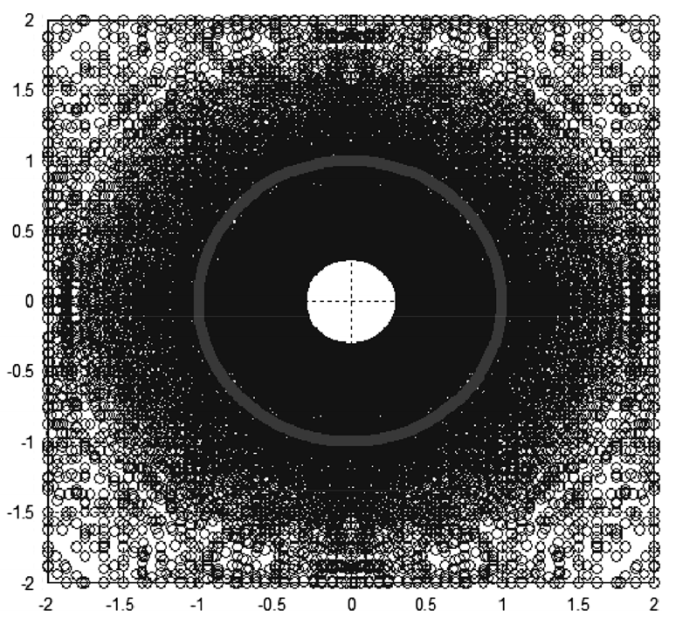
\includegraphics[width=0.6\linewidth]{Images/RevisaoDeLiteratura/CordicComparationMSR.PNG}
	\caption{MSR com I=2, J=1 e N=2}
	\vspace{-3.5mm}
	\caption*{Fonte: \cite{Chih}}
	\label{fig:CordicComparationMSR}
\end{figure}    
\vspace{5mm}

O incremento de mais termos SPT na defini��o do �ngulo de rota��o $\theta_n$ acaba por dar ao conjunto dos �ngulos elementares mais liberdade combinacional dentro do c�rculo unit�rio. No algoritmo CORDIC tradicional e no EEAS havia uma dificuldade de realizar rota��es maiores que $\pi / 4$, devido a distribui��o  dos �ngulos elementares, como pode ser visto nas Figura (\ref{fig:CordicComparationCordic}) e (\ref{fig:CordicComparationEEAS}). Devido a esta dificuldade era necess�rio realizar uma pr�-rota��o no vetor de entrada, quando o �ngulo de rota��o era maior que $\pi / 4$, a fim de reduzir o �ngulo para uma faixa mais aceit�vel de rota��o, o que aumenta o custo computacional do algoritmo, e demandava mais recursos de \textit{hardware}. No algoritmo MSR o conjunto dos �ngulos elementares no circulo unit�rio � maior e melhor distribu�dos como visto na Figura (\ref{fig:CordicComparationMSR}). Isto possibilita ao MSR alcan�ar �ngulos de rota��o de $0$ � $2 \pi$, varrendo todo o circulo unit�rio.

O desempenho do algoritmo EEAS, como mostrado na se��o anterior, � diretamente relacionado com a escolha dos par�metros CORDIC $\mu_{0}$, $\mu_{1}$, $s_0$ e $s_1$. De maneira an�loga � a determina��o dos par�metros CORDIC $J$, $I$, $\mu_{i}$, $\mu_{j}$, $s_i$ e $s_j$ que garante a converg�ncia e efici�ncia do algoritmo. 

Para determinar os par�metros Cordic do algoritmo MSR, \citeonline{Chih} utiliza a an�lise do erro entre o vetor idealmente rotacionado, e o vetor que na pr�tica do Algoritmo MSR consegue alcan�ar no rotacionamento. Para exemplificar, considere que se deseja rotacionar um vetor $\overline{OD}$ pelo �ngulo $\theta$ at� a posi��o do ponto $A$, formando assim um novo vetor rotacionado $\overline{OA}$. Considerando que o MSR n�o consiga rotacionar o vetor $\overline{OD}$ por exatamente $\theta$, e que devido ao ganho Cordic o m�dulo do vetor rotacionado seja diferente do vetor $\overline{OD}$. Logo, a nova posi��o do vetor rotacionado � $\overline{OB}$, como mostrado na Figura (\ref{fig:AnaliseDoErroZeta})\cite{Chih}.

\vspace{5mm}
\begin{figure}[H]
	\centering
	\captionsetup{width=0.45\textwidth, font=footnotesize, textfont=bf}	
	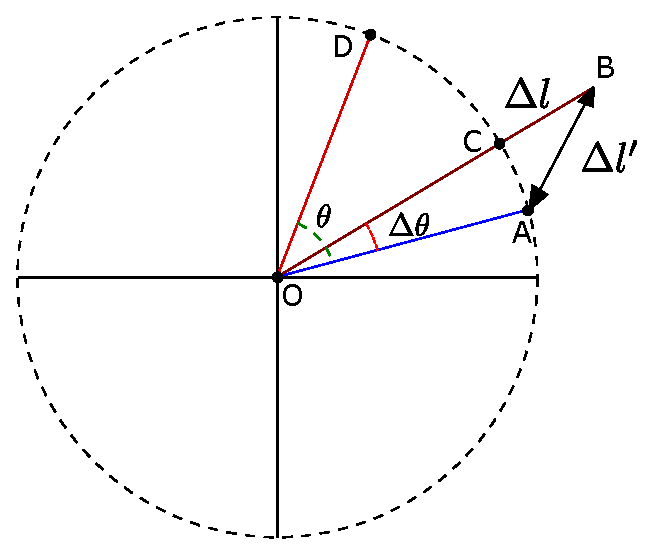
\includegraphics[width=0.45\linewidth]{Images/RevisaoDeLiteratura/AnaliseDoErroZeta.eps}
	\caption{MSR com I=2, J=1 e N=2}
	\vspace{-3.5mm}
	\caption*{Fonte: \cite{Chih}}
	\label{fig:AnaliseDoErroZeta}
\end{figure}    
\vspace{5mm}

Analisando a Figura (\ref{fig:AnaliseDoErroZeta}), o erro de aproxima��o $\upepsilon$ do algoritmo MSR � representado pelo trecho $\overline{OB}$, denominado $\Delta l'$. J� o erro angular � representado por $\Delta \theta$, e o erro do m�dulo � representado pelo trecho $\overline{OC}$, denominado $\Delta l'$. Segundo \citeonline{Chih}, quando $\Delta \theta$ � suficientemente pequeno � poss�vel obter a seguinte express�o:

\begin{eqnarray}
	\Delta l'^2 ~ = ~ \overline{OA}^2 + \overline{OB}^2 - 2\overline{OA} \times \overline{OB}cos(\Delta \theta), \\
	\Delta l'^2 ~ = ~ 1 + (1 + \Delta l)^2 - 2 \times 1 \times (1+\Delta l) \times \sqrt{1 - sin^2 (\Delta \theta)},\\
	\Delta l'^2 ~ \approx ~ \Delta l^2 + \Delta \theta^2.
	\label{eq:AproximacaoDeltal} 
\end{eqnarray}

Por meio de (\ref{eq:AproximacaoDeltal}) � poss�vel concluir que o erro angular $\Delta \theta$, e o erro modular $\Delta l$ possuem o mesmo impacto no erro de aproxima��o do algoritmo MSR. Portanto, afim de otimizar o desempenho do algoritmo MSR � necess�rio escolher um conjunto de par�metros CORDIC que privilegiem igualmente a redu��o de ambos os erros de aproxima��o \cite{Chih}.

Assim determinar o conjunto dos melhores valores para os par�metros CORDIC $J$, $I$, $\mu_{i}$, $\mu_{j}$, $s_i$ e $s_j$ nada mais � do que uma tarefa de otimiza��o, onde a equa��o de minimiza��o � a express�o do erro $\upepsilon$, o qual pode ser definido como:

\begin{equation}
	min~ \upepsilon~ = ~\sqrt{\Delta l^2 + \Delta \theta^2}
	\label{eq:OtimizacaoMSR}.
\end{equation}

Para solucionar esta tarefa de otimiza��o de $\upepsilon$  � poss�vel utilizar diferentes tipos de algoritmos, e inclusive adaptar o algoritmo TBS j� apresentado. Segundo \citeonline{Chih}, existe uma certa restri��o quanto a utiliza��o de algoritmos como o \textit{greedy}, pois este tipo de algoritmo Guloso n�o garante a melhor solu��o dentro do conjunto de solu��es poss�veis deste problema.

\subsubsection{An�lise do Erro}
\label{section:AnaliseDoErro}

Um importante fator para a determina��o do melhor conjunto de par�metros Cordic para o MSR, al�m da minimiza��o do erro  $\upepsilon$, � o efeito do ru�do de arredondamento (\textit{Roundoff Noise Analysis}) $e_n$, e o erro de \textit{overflow}, ou estouro da palavra bin�ria. Ambos os efeitos ocorrem ao longo das opera��es l�gicas promovidas pelo algoritmo CORDIC, em especial devido a opera��o de compensa��o do ganho $K_c$. Esta compensa��o envolve uma opera��o de multiplica��o, o que acentua os problemas de arredondamento da parte fracion�ria e, dependendo do valor da compensa��o, pode causar um \textit{overflow} da palavras bin�ria.

Nos dispositivos digitais o n�mero de \textit{bits} utilizados para representar sinais quantizados � limitado de acordo com a arquitetura. Este limite de representa��o acaba por impactar na resolu��o da palavra bin�ria para n�meros fracion�rios, o que for�a a realiza��o de arrendondamentos na representa��o bin�ria. 

Para representar o conjunto dos n�meros racionais no mundo digital, a arquitetura dos sistemas digitais reserva parte dos \textit{bits} da palavra bin�ria para representar o fracion�rio do n�mero racional. Assim, segundo \citeonline{Chih},  os n�veis de quantiza��o para um sinal digital s�o definidos como:

\begin{equation}
	\left\{-2^{W-i-1},...,-2^{-i+1}, -2^{-i}, -2^{-i+1}, ..., 2^{W-i-1} \right\}.  
\end{equation}

Onde $W$ representa o numero de \textit{bits} da palavra bin�ria, e $i$ representa o n�mero de d�gitos fracion�rios.

Uma solu��o simples para reduzir o efeito do $e_n$ � aumentar o n�mero de \textit{bits} $W$ e $i$, melhorando a resolu��o da representa��o. Por�m, esta solu��o, como afirma \cite{Chih}, provocaria uma redu��o na velocidade computacional do sistema, e ainda consumiria mais recursos de \textit{hardware}. Outra op��o seria reduzir o n�mero de \textit{bits} utilizados para representar a parte inteira do n�mero, e transferir estes \textit{bits} para a parte fracion�ria. Por�m, este m�todo pode provocar um \textit{overflow} da palavra bin�ria, o que � ainda pior do que um ru�do de arredondamento.  

Considerando a amplitude $\rho$ de um sinal de entrada, definido entre os intervalos:

\begin{equation}
	-2^{Wa} \leq \rho \leq 2^{W_b} -1,~~para~W_a,W_b \geq 0,
\end{equation} 

onde $Wa$ e $Wb$ representam respectivamente o limite superior e inferior da amplitude do m�dulo deste sinal. Ainda:

\begin{equation}
	W_{max}~=~max\{W_a,W_b\}.
\end{equation} 
 
Como o limite absoluto deste sinal. O n�mero m�nimo de \textit{bits} necess�rios para representar este sinal seria de $(W_{max}+1)$. Assim, segundo \citeonline{Chih}, para evitar um \textit{overflow} seria necess�rio manter o sinal de entrada dentro da seguinte restri��o:

\begin{equation}
	2^{W_{max}}~\leq~2^{W-1-i}.
\end{equation}

Para solver o problema do ru�do de arredondamento, \citeonline{Chih} assumem que o $e_n$ � uniformemente distribu�do e n�o possui correla��o com outros sinais. Al�m de considerar que, baseado nos n�veis de quantiza��o, o $e_n$ est� situado em uma faixa sim�trica de $(-2^{-i-1}, 2^{-i-1})$. Portanto, a vari�ncia de $e_n$ � dada por:

\begin{equation}
	\sigma_{e_n}^2~=~\frac{V^2_{LSB}}{12},
	\label{eq:variancia}
\end{equation} 

onde  $V_{LSB}$ � igual a $2^i$. Logo, a vari�ncia do erro de arredondamento � proporcional ao quadrado valor do ultimo $bit$ da palavra bin�ria. 

Como base em (\ref{eq:variancia}), \citeonline{Chih} analisam o efeito a opera��o de rota��o tem sobre a vari�ncia de $e_n$, e mais especificamento o efeito que o ganho $K_c$ tem sobre o SQNR. Quando o ganho $K_c$ � $> ~1$ ou $<~1$ SQNR � reduzido para $1/(K_n)$ a cada itera��o CORDIC.

O ganho $K_C$ � fator importante no projeto dos par�metros Cordic para o MSR, afetando tanto o erro $e_n$ quanto $\upepsilon$. Para refinar a fun��o de minimiza��o apresentada em (\ref{eq:OtimizacaoMSR}), \citeonline{Chih} adicionam a seguinte restri��o em rela��o ao valor do ganho $K_c$:

\begin{equation}
	P_{lower} ~=~1/P_{upper},
\end{equation}

onde $P_{upper}$ e $P_{lower}$ s�o, respectivamente, o limite superior e o limite inferior de $K_n$ a cada intera��o.

O gr�fico da Figura (\ref{fig:RelacaoSQNReKc}) mostra uma an�lise pr�tica entre o n�vel do SQNR e o $P_{upper}$, para diferentes valores de deslocamento de \textit{bits} ($S$). Por meio desta an�lise \citeonline{Chih} sugerem que para um bom projeto de par�metros MSR Cordic, onde $N_{spt}~=~3$ e $N=3$, o valor de  $P_{upper}$ deve estar pr�ximo de $1,5$. J� que, como pode ser visto na Figura (\ref{fig:RelacaoSQNReKc}), para valores maiores o desempenho de SQNR � saturado. Logo, para este caso, � poss�vel adicionar mais esta restri��o a equa��o de minimiza��o do erro $\epsilon$.

\vspace{5mm}
\begin{figure}[H]
	\centering
	\captionsetup{width=0.9\textwidth, font=footnotesize, textfont=bf}	
	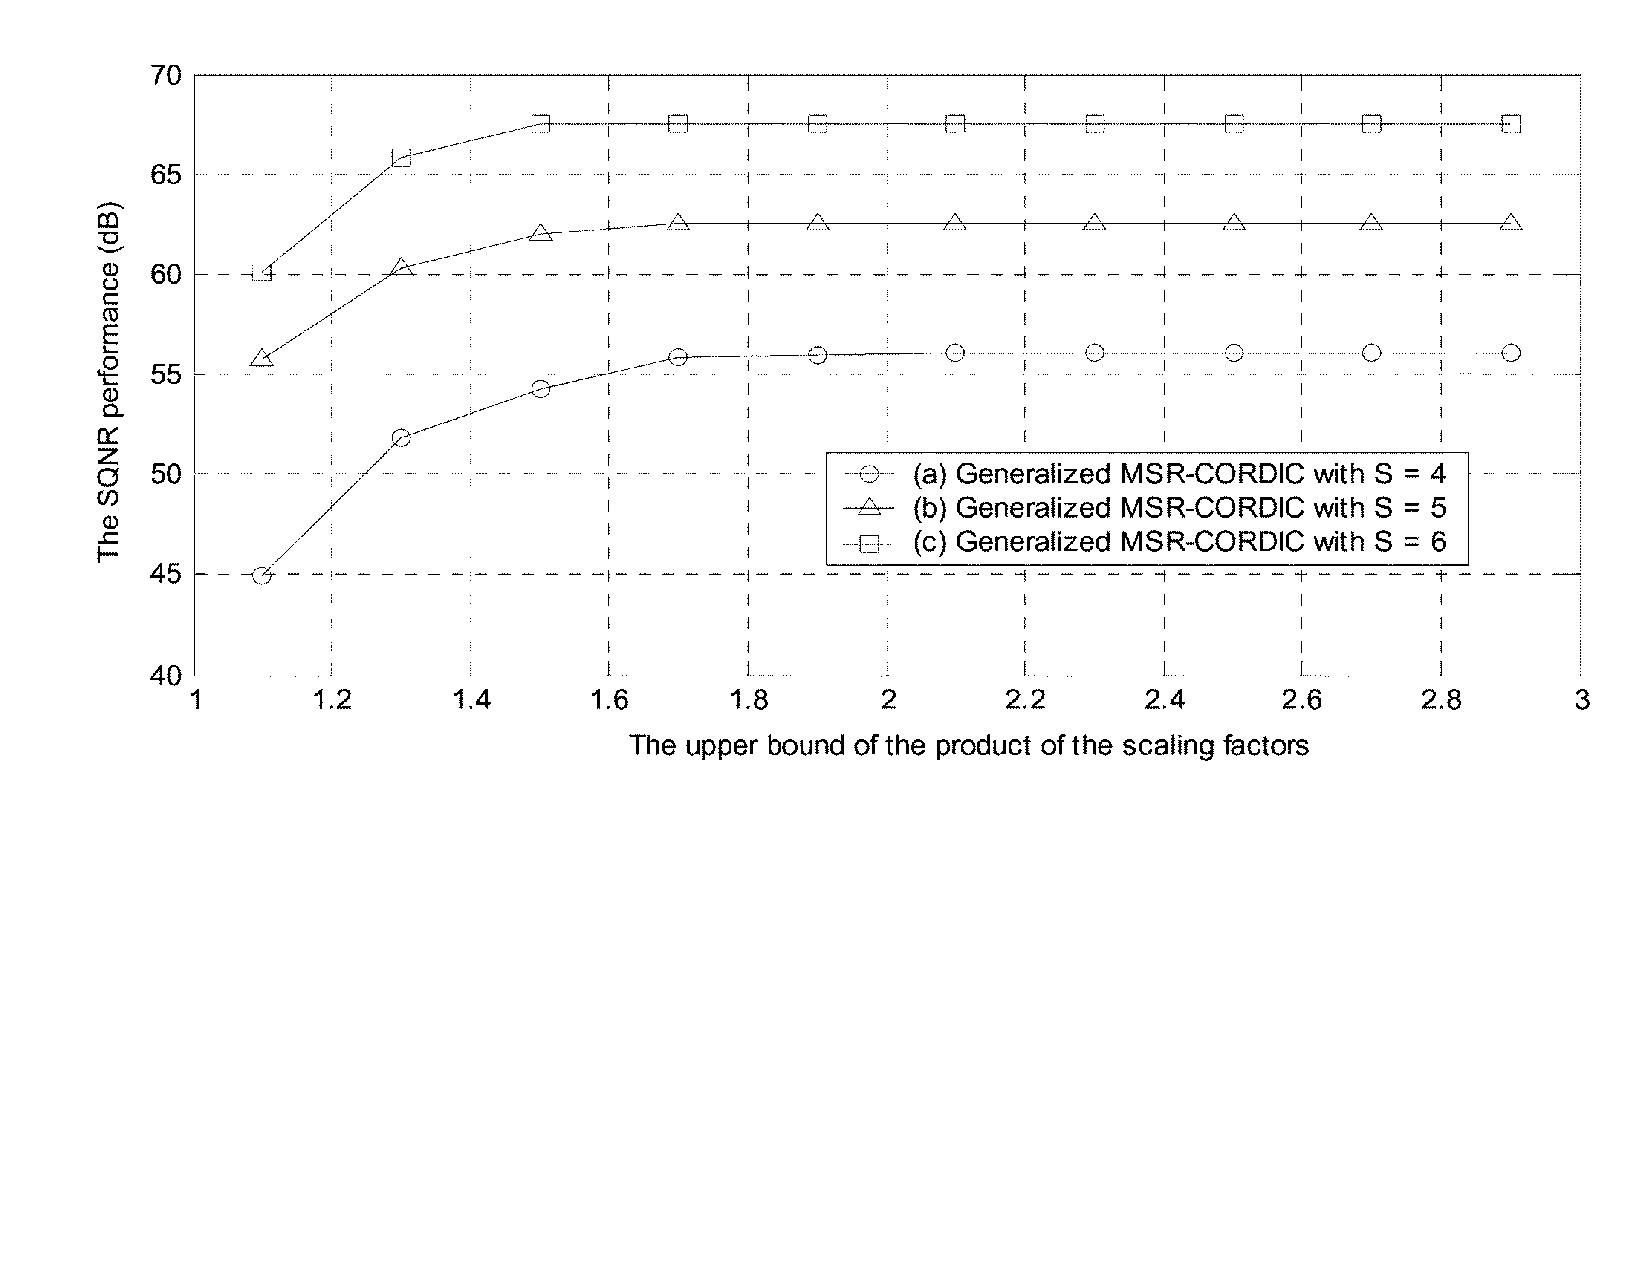
\includegraphics[width=0.9\linewidth]{Images/RevisaoDeLiteratura/RelacaoSQNReKc.pdf}
	\caption{Rela��o entre o $P_{upper}$ e o SQNR para MSR-CORDIC, como $N_{spt}~=~3$ e $N=3$}
	\vspace{-3.5mm}
	\caption*{Fonte: \cite{Chih}}
	\label{fig:RelacaoSQNReKc}
\end{figure}    
\vspace{5mm}

O �ltimo aspecto da melhoria do erro $e_n$ � a escola dos par�metros $I$ e $J$. Estes par�metros est�o diretamente relacionados a $N_{spt}$, o n�mero de termos SPT presentes na equa��o $x(n+1)$ e $y(n+1)$. Esta rela��o � descrita por (\ref{eq:Nspt}). O valor de $N_{spt}$ � uma escolha que impacta na no n�mero de deslocadores de \textit{bits} (\textit{shifters}) necess�rios para realizar a opera��o Cordic, sendo mais comum na bibliografia observar implementa��o MSR Cordic com $N_{spt}=3$ ou $N_{spt}=4$ \cite{Park} \cite{Chih} \cite{Meher}. 

Os valores $I$ e $J$ podem ser escolhidos como fixos (Modo Normal) ou podem ser din�micos a cada opera��o de rotacionamento (Modo Generalizado). Tanto no modo Normal quanto o modo Generalizado, o valor de $I$ e $J$ devem obedecer a restri��o $I+J=N_{SPT}$, por�m ao utilizar o modo Normal � poss�vel reduzir a complexabilidade do \textit{hardware} e alcan�ar um desempenho aceit�vel. Para tal, quando em modo de opera��o Normal, os par�metros deve $I$ e $J$ devem atender a duas restri��o dadas a seguir \cite{Chih}:

\begin{itemize}
	\item Se $N_{spt}$ � par: $I~=~J~=~N_{spt}/2$,
	\item Se $N_{spt}$ � �mpar: $J~=(N_{spt}+1)/2$ e $I~=~J-1$.
\end{itemize}

A opera��o em modo Generalizado permite que o desempenho do MSR Cordic seja maior, j� que nesta configura��o as possibilidades combinat�rias dos par�metros Cordic s�o maiores. Neste modo passa a existir, al�m da opera��o normal de rotacionamento, a possibilidade de ocorrer a opera��o de multiplica��o de escala, quando $J=0$, e a opera��o de invers�o de escala, quando $I=0$. Estas opera��es adicionais maximizam o desempenho nas rota��es em �ngulos como $\pi/4$, $\pi/2$ e $\pi$. Na pr�tica, este modo requer o uso de mais 3 \textit{switches} de controle, o que em muitas aplica��es torna vi�vel aumentar o consumo de recursos para alcan�ar um melhor desempenho. 

Alinhando todas as restri��es apresentadas com a equa��o de minimiza��o apresentada em (\ref{eq:OtimizacaoMSR}), � obtido um conjunto de par�metros Cordic que otimizam a opera��o de rotacionamento, elevando o valor de SQNR do sinal.



   
   
  
	
\section{Zynq-7000}
	\subsection{FPGA}

\citeonline[p.~4]{Moore} define a FPGA como um dispositivo semicondutor capaz de ser totalmente redefinido ap�s sua fabrica��o, permitindo ao programador reconfigurar produtos e fun��es j� implementadas, adaptando o \emph{hardware} a novas fun��es. De forma pr�tica, a FPGA permite uma flexibilidade em um projeto, podendo mudar a forma como ele � implementado, sem a necessidade de se construir um \emph{hardware} novo. 

Para \citeonline[p.~4]{Moore}, comparado com as outras formas de construir um hardware, a FPGA oferece duas grandes vantagens em uma aplica��o. Primeiro, para uma aplica��o ao inv�s de se utilizar um circuito integrado padr�o comercial, que geralmente �  super ou subdimensionado, ou ainda desenvolver um novo projeto de circuito integrado especifico, consumindo tempo e recursos, a FPGA  possibilita desenvolver um \textit{hardware} exatamente dentro das especifica��es, personalizado e otimizado para a fun��o destinada. Em segundo, por�m t�o importante quanto, � que essa capacidade de personaliza��o de \textit{hardware} possibilita a realiza��o de opera��es de modo mais simplificado, r�pido e energeticamente eficiente se comparado a um microprocessador.

As FPGAs s�o baseadas em unidades l�gicas elementares b�sicas, ou BLEs (\textit{Basic Logic Elements}), dentro de uma hierarquia de interconex�es reconfigur�veis que permitem que os LEs sejam fisicamente conectados uns aos outros de diferentes formas criando uma enorme variedade de componentes digitais. A arquitetura das FPGAs modernas s�o constitu�das basicamente por conjunto de mem�rias de armazenamento em massa SRAM (\textit{Static Random Access Memory}), Portas de Entrada/Sa�da, blocos l�gicos configur�veis CLB (\textit{Configurable Logic Blocks}) e sistema de roteamento, como pode ser visto na Figura (\ref{fig:FPGAArchitecture}) \cite[p.~5]{Moore}. 

\vspace{8mm}
\begin{figure}[H]
	\centering
	\captionsetup{width=0.5\textwidth, font=footnotesize, textfont=bf}	
	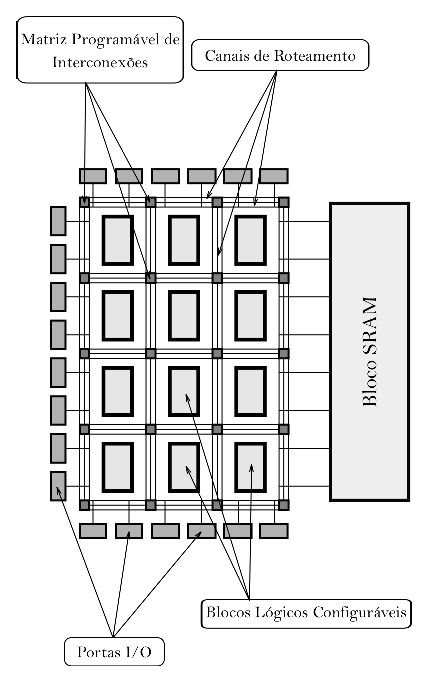
\includegraphics[width=0.5\linewidth]{Images/RevisaoDeLiteratura/FPGAArchitecture.eps}
	\caption{Arquitetura Tipica de uma FPGA}
	\vspace{-3.5mm}
	\caption*{Fonte: Adaptado \citeonline[p.~6]{Meyer}}
	\label{fig:FPGAArchitecture}
\end{figure}
\vspace{8mm}

Os  CLB s�o blocos realizam opera��es logicas b�sicas e armazenam pequenos volumes de dados. Comumente as opera��es complexas, necess�rias para o processamento de uma aplica��o, s�o divididas em processos mais simples para cada uma das CLBs selecionadas, de modo que a soma das tarefas de cada CLB seja equivalente a opera��o complexa, em uma estrat�gia de divis�o e conquista. Para realizar opera��es l�gicas b�sicas e ainda armazenar pequenos volumes de dados os CLBs tecnicamente poderiam ser apenas um pequeno circuito de transistores (granularidade fina), ou at� mesmo um processador completo (granularidade grosseira). Se os CLBs fossem granularidade fina, para realizar tarefas complexas seria necess�rio um grande n�mero de CLBs e um sistema de roteamento complexo para interconecta-los, o que resultaria em uma FPGA de baixa performance e um elevado consumo energ�tico. Por outro lado de as CLBs forem de uma granularidade mais grosseira seria um desperd�cio de recurso utiliza-los em opera��es mais simples \cite[p.~11]{tree}. Assim a escolha do n�vel de complexabilidade, ou granula��o, das CLBs de uma FPGA � um compromisso de otimiza��o de recursos.

Ainda segundo \citeonline[p.~11]{tree} dentro da grama de granula��o das CLBs, algumas arquiteturas incluem o uso de portas NAND, interconex�o de multiplexadores e tabelas de busca LUT (\textit{Lookup Table}). Em especial fabricantes como a Xilinx utilizam CLBs baseadas em LUTs, j� que CLBs baseadas em LUT oferecem uma boa rela��o de granula��o, otimizando os recursos da FPGA para aplica��es simples at� as mais complexas. Este tipo de CLB  pode incluir uma �nico elemento logico b�sico BLE (\textit{Basic Logic Element}), ou mesmo um \textit{cluster} de BLEs interconectados, como mostrado na Figura (\ref{fig:ArchitectureClusterBLE}).

\vspace{6mm}
\begin{figure}[H]
	\centering
	\captionsetup{width=0.4\textwidth, font=footnotesize, textfont=bf}	
	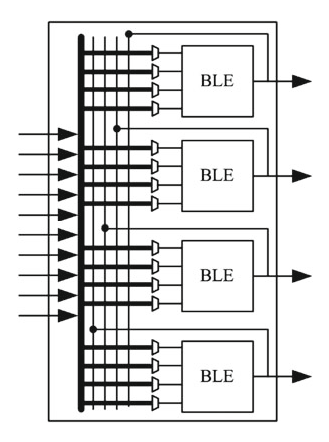
\includegraphics[width=0.4\linewidth]{Images/RevisaoDeLiteratura/ArchitectureClusterBLE.eps}
	\caption{Arquitetura de uma CLB com 4 BLEs}
	\vspace{-3.5mm}
	\caption*{Fonte: Adaptado \citeonline[p.~13]{tree}}
	\label{fig:ArchitectureClusterBLE}
\end{figure}
\vspace{6mm}

Segundo \citeonline[p.~11]{tree}, um BLE mais simples consiste basicamente de um LUT e um \textit{Flip-Flop} tipo D, como pode ser visto na Figura (\ref{fig:BasicLogicElement}). Um LUT com $k$ entradas pode implementar $k$ fun��es booleanas utilizando os espa�os de mem�ria SRAM dentro da LUT. O exemplo apresentado na Figura (\ref{fig:BasicLogicElement}) utiliza  16 bits de mem�ria SRAM, os quais s�o conectadas a entrada do multiplexador que possui 4 bits de sele��o, e cuja sa�da � ligada ao \textit{flip-flop}. Esta configura��o permite que a LUT tenha $2^k$ combina��es das $k$ opera��es booleanas. 

\vspace{6mm}
\begin{figure}[H]
	\centering
	\captionsetup{width=0.5\textwidth, font=footnotesize, textfont=bf}	
	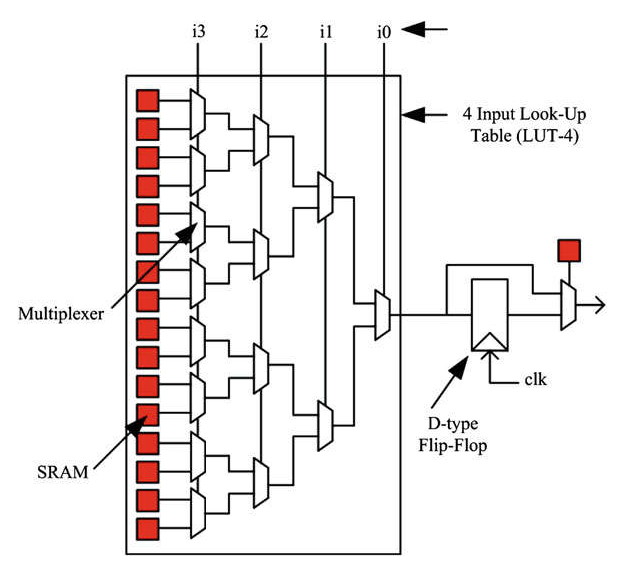
\includegraphics[width=0.5\linewidth]{Images/RevisaoDeLiteratura/BasicLogicElement.eps}
	\caption{Arquitetura de uma BLE (\textit{Basic Logic Element})}
	\vspace{-3.5mm}
	\caption*{Fonte: Adaptado \citeonline[p.~13]{tree}}
	\label{fig:BasicLogicElement}
\end{figure}
\vspace{6mm}

Um �nico BLE � capaz de realizar algumas opera��es booleanas b�sicas, por�m em clusters as combina��es de opera��es aumentam. FPGAs modernas tipicamente cont�m de 4 a 10 BLEs em um �nico cluster. Por�m estas FPGAs n�o possui apenas BLEs id�nticas, na verdade h� uma grande heterogenia de blocos, sendo muitos deles desenvolvidos para prop�sitos espec�ficos. Entre estes blocos de prop�sito espec�fico est�o multiplicadores, somadores, mem�rias e DSPs (\textit{Digital Signal Processor}), entre outros. Estes blocos s�o desenvolvidos para otimizar o espa�o, processamento, roteamento e demais recursos de \textit{hardware} que seriam necess�rios para implementar as mesmas fun��es em BLEs comuns, sendo essenciais em certas aplica��es.

Para \cite{Ibrahim}, a FPGA � uma boa escolha para a implementa��o do algoritmo da FFT  devido a grande variedade de recursos de hardware sintetiz�veis, al�m de possuir recursos de programa��o paralela que permite o processamento paralelo de sinais, conferindo assim uma maior rapidez na execu��o do algoritmo. Como afirma \citeonline[Pref�cio]{Meyer}, muitos algoritmos de processamento de sinais, como FFT (\emph{Fast Fourier Transform}) e os filtros FIR ou IIR,  implementados anteriormente em Circuitos Integrados de Aplica��o Especifica ou ASIC (\emph{Application Specific Integrated Circuits}), agora est�o sendo implementados em FPGAs.

O dispositivo escolhido para a implementa��o do algoritmo Radix-2 � o kit de desenvolvimento para FPGA denominado $Spartan^\circledR -3E~FPGA~Starter~Kit~Board$, apresentado na figura (\ref{fig:Sparta-3E-FPGA- StarterKitBoard}). Tal kit possui uma FPGA XC3S500E, com  1.164 CLBs,  4.656 \emph{slices}, um bloco de RAM de 360 Kbits, 20 multiplicadores dedicados e 232 portas de entrada e sa�da utiliz�veis \cite{DataSheet}.

%\begin{figure}[H]
%	\centering
%	\captionsetup{width=0.6\textwidth, font=footnotesize, textfont=bf}	
%	\includegraphics[width=0.6\linewidth]{Images/Sparta-3E-FPGA-StarterKitBoard.eps}
%	\caption{$Spartan^\circledR -3E~FPGA~Starter~Kit~Board$}
%	\vspace{-3.5mm}
%	\caption*{Fonte: \citeonline{DataSheet}}
%	\label{fig:Sparta-3E-FPGA- StarterKitBoard}
%\end{figure}

\subsection{Zynq 7000}

\subsection{ZynqBerry TE0726-03M}
